\documentclass[a4j,12pt,onecolumn,oneside,notitlepage,openany,jarticle,final]{jreport}%両面刷り
%
\usepackage[dvipdfmx]{graphicx}
\usepackage{cite}
\usepackage{makeidx,graphicx,epsbox,delarray}
\usepackage{fancyhdr,hhline,array}
\usepackage{pifont}
\usepackage{amssymb}
\usepackage{subfigure}
\usepackage{multirow}
\usepackage[dvipdfmx]{}
\usepackage{otf}
\usepackage{here}
\usepackage{url}


\renewcommand{\bibname}{参考文献}
\bibliographystyle{junsrt} 
%余白の設定 A4は縦297mm 横210mm 初期余白25.4mm
\topmargin=4.6mm %上余白 ヘッダをいれて30mmにする(4.6=30-25.4)その後微調整
\oddsidemargin=6.6mm %左余白 40mm=25.4+14.6
\textwidth=158mm %適当に決めました(155=210-40-15)
\textheight=252.5mm %同様に↑(232=297-40-25)
\makeindex
\date{}
%ページ番号を各ページ下に表示
\pagestyle{fancy}
% ヘッダの下線を引かない。
\lhead{}
\chead{}
\rhead{}
\renewcommand{\headrulewidth}{0.0pt}
\renewcommand{\footrulewidth}{0.0pt}
%以下「\UTF{2460}」等の囲い文字を使うための新しいコマンドを定義
\newcommand{\MARU}[1]{{\ooalign{\hfil#1\/\hfil\crcr
\raise.167ex\hbox{\mathhexbox20D}}}}
%
% 本文の行数と桁数を指定出来るように
\def\linesparpage#1{\baselineskip=\textheight
\divide\baselineskip by #1}
\def\kcharparline#1{%
\ifx\xkanjiskip\undefined%
% NTT jTeX用
\jintercharskip 0mm plus 0.2mm minus 0.2mm
\else
% ASCII pTex用
\xkanjiskip 0mm plus 0.2mm minus 0.2mm
\fi
\settowidth{\textwidth}{}%
\multiply\textwidth by #1}
%
%%% Document Start %%%%%%%%%
%
\begin{document}
%タイトルページ
\begin{titlepage}
\begin{center}
%
\vspace{20pt}
{\fontsize{50pt}{0pt}\selectfont \bf 関西大学 \\ \vspace{12pt} システム理工学部 \\ \vspace{12pt} 卒業論文} \\ %タイトル
\vspace{50pt}
%
{\fontsize{25pt}{0pt}\selectfont \underline{2022年度}} \\
\vspace{30pt}
{\fontsize{25pt}{0pt}\selectfont \bfseries
	\underline{対話型進化計算} \\
	\vspace{7pt}
	\underline{性格特性表現} \\
	\vspace{7pt}
	\underline{ロボットジェスチャ最適化}
} \\
\vspace{30pt}
%
{\fontsize{22pt}{0pt}\selectfont 電気電子情報工学科} \\
\vspace{30pt}
{\fontsize{22pt}{0pt}\selectfont \underline{学籍番号 電19-0188} \\}
\vspace{15pt}
\underline{{\fontsize{22pt}{0pt}\selectfont 氏 名}\hspace{11pt}{\fontsize{30pt}{0pt}\selectfont 三河 亮斗}} \\
\vspace{15pt}
\underline{{\fontsize{22pt}{0pt}\selectfont 指導教授}{\fontsize{30pt}{0pt}\selectfont \hspace{5zw}}{\fontsize{12pt}{0pt}\selectfont 印}} \\
\vspace{25pt}
%
\fbox{{\fontsize{28pt}{0pt}\selectfont 感性情報システム研究室}} \\
\end{center}
\end{titlepage}
%フォントサイズと行間を指定
\fontsize{12pt}{21pt}
\selectfont
% 一ページを30行に
\linesparpage{30}
%タイトルと要旨はページ番号を出力しない
\pagestyle{empty}
%
\topmargin=-20.6mm %上余白 ヘッダをいれて30mmにする(4.6=30-25.4)その後微調整
\oddsidemargin=6.6mm %左余白 40mm=25.4+14.6
\textwidth=155mm %適当に決めました(155=210-40-15)
\textheight=252.5mm %同様に↑(232=297-40-25)
%目次のページ番号をローマ数字に指定
\addtolength{\textheight}{-12truemm}
\setcounter{page}{1}
\pagenumbering{roman}
\pagestyle{fancy}
%目次出力
\tableofcontents

\topmargin=-8.6mm %上余白 ヘッダをいれて30mmにする(4.6=30-25.4)その後微調整
\oddsidemargin=6.6mm %左余白 40mm=25.4+14.6
\textwidth=155mm %適当に決めました(155=210-40-15)
\textheight=240.5mm %同様に↑(232=297-40-25)

% !TEX root = MasterPaper.tex
\chapter{序論}
\thispagestyle{fancy}
\lhead{}
\chead{}
\rhead{}
\lfoot{} 
\cfoot{\thepage}  
\rfoot{}
%目次のページ番号をアラビア数字に指定
\setcounter{page}{1}
\pagenumbering{arabic}

近年世界で流行している新型コロナウイルス(COVID-19)の影響により,現地でのスポーツ観戦が困難になっている.
それに伴って,現地での観戦時特有の「臨場感」が失われてしまっていることが大きな問題となっている.

この問題を受け,近年ではKDDIと横浜DeNAベイスターズが実施するバーチャルハマスタなどの,次世代型のスポーツ観戦方式が登場している\cite{hamasuta}.
バーチャルハマスタとは,バーチャル空間にスタジアムを構築し,自宅からスマートフォンやパソコン,VRデバイスを使って観戦体験ができるプロジェクトである.
VR空間で,ユーザはオリジナルのアバターを用いて多くのファンと一緒に観戦し,コミュニケーションをとりながら球場の雰囲気を楽しむことができる.

しかし,この観戦方式は,観戦時にアバターが棒立ちになってしまうことや,感情表出方法が絵文字による表出のみであることから,現地でのスポーツ観戦を再現しきれておらず,臨場感を演出できていないと考えられる.
ここで,VR空間における棒立ちのアバターを感情表出を行うロボットに置き換えることで,現地でのスポーツ観戦を再現できる可能性がある.

一方で近年,自動運転を搭載した自動車が発表されるなど,人工知能を搭載した製品の普及は目覚ましいものとなっている.
使用者の暮らしに応じた機能を提示する人工知能搭載型の様々な電化製品が開発され,人工知能を搭載したロボットが囲碁でプロの棋士に勝利するなど,人工知能は人々にとって身近な存在になりつつある\cite{healsio}\cite{go}.

また,近年ではロボットに人工知能を搭載し,人とコミュニケーションをとるロボットが数多く登場している.
このようなロボットはコミュニケーションロボットと呼ばれており,その代表的なものにパーソナルロボットやペットロボットが挙げられる\cite{toyota}\cite{aibo}.
これらのロボットは人の心的状況を読み取り,感情的なコミュニケーションをとることが求められる.
さらに今後,公共の場で人の代わりにコミュニケーションをとるロボットが普及することが示唆されている\cite{deep}.

このようなコミュニケーションロボットは人と円滑なコミュニケーションを行うため,非言語情報による感情表現が重要だと言われている.
現在でも,顔表情で感情表出を行うロボットや,指と手によるジェスチャーとして手話を取り上げ,ロボットに実装した例が報告されている
\cite{kao}\cite{syuwa}.
コミュニケーションにおいて,人間に心的作用をもたらす要因は主として非言語情報である\cite{higengo}.
非言語コミュニケーションの重要性は,人間同士だけでなく,人間とロボットの場合においても同様であると考えられる.
したがって,人間と共存するコミュニケーションロボットには,非言語機能が必要になると考えられる.
そこで本研究では,非言語情報によって感情表出を行うロボット集団との試合観戦は,臨場感を演出できるか検証する.

本論文は5章で構成される.

第2章では,臨場感についての関連研究,スポーツ観戦における臨場感及び感性とロボットの関係性について述べる.
初めに,臨場感の定義と臨場感を感じる事象である「興奮」や「面白さ」の高まりに関する先行研究について述べる.
次に,スポーツ観戦における臨場感の演出に必要な要素について述べる.
最後に,ロボットに感性を導入する意義,ロボットと人間とのインタラクションについて述べる.

第3章では,スポーツ観戦における臨場感演出の定義,本研究で提案する内部モデルについての詳細及び実験環境,及び実験におけるロボット集団の動作について述べる.
本研究ではロボットが試合観戦中に感情表出をしているように見せる内部モデルを提案する.
また,本実験で用いたロボット集団とインタラクションをとる仮想環境と,仮想環境でのロボットの動作について述べる.

第4章では,提案ロボット集団との試合観戦が臨場感を演出できるか検証するための実験について述べる.
評価実験では,被験者は提案ロボット集団と比較ロボット集団の2集団と試合観戦を行い,アンケートによって試合観戦における臨場感,及びロボット集団への評価を行う.

第5章は結論であり,本研究により得られた成果についてまとめると共に,今後に残された課題について述べる.



% !TEX root = MasterPaper.tex
\chapter{先行研究}
\thispagestyle{fancy} % このページのみ
\lhead{}
\chead{}
\rhead{}
\lfoot{} 
\cfoot{\thepage}  
\rfoot{}
%

\section{遺伝的アルゴリズム}
\label{sec2.1}

\subsection{遺伝的アルゴリズムの概要}
\label{sec2.1.1}

GAとは選択淘汰や突然変異など生物進化の仕組みを模範した最適化アルゴリズムである.GAは1975年にJ.H.Hollandnによって提案された手法である.GAの枠組みはとても簡単であり,与えられた最適化問題の評価関数に対して,いくつかの乱数と単純な記号処理を用いるだけで求めることができる.また,GAは他の最適化アルゴリズムより比較的少ない計算量で最適解を求めることができる.

GAのフローチャートを図2.1に示す.GAでは,生成した遺伝子列に対して,選択,交叉,突然変異といった生物進化の仕組みを模した処理を行う.問題の解候補を生物集団の各個体と呼び,各個体のパラメータを遺伝子と呼ぶ.

以下に図2.1の具体的な流れについて述べる.


\begin{description}
\item[ (1) ]遺伝子型の決定

GAの対象となる問題を遺伝子列に変換する.

\item[ (2) ]初期遺伝子集団の決定

(1)で決められた遺伝子型で,要素の異なるさまざまな個体をランダムに発生させる.

\item[ (3) ]適応度評価

生成された遺伝子集団に対して評価を行い,各個体の適応度をあらかじめ定められた計算方法と評価で算出する.

\item[ (4) ]選択処理

遺伝子集団中における各個体の適応度に基づいて,交叉処理を行う個体を選択する.

\item[ (5) ]交叉処理

(4)で選択された2つの個体間で遺伝子を組み替えて新しい個体を発生させる.

\item[ (6) ]突然変異処理

遺伝子のある部分を特定の確率で強制的に変化させる.

\item[ (7) ]終了条件(遺伝子集団の評価)

生成された次世代の遺伝子集団が,GA処理を終了するための評価基準を満足しているかどうかを確認する.
\end{description}

\begin{figure}[p]
\begin{center}

\vspace{1.5cm}
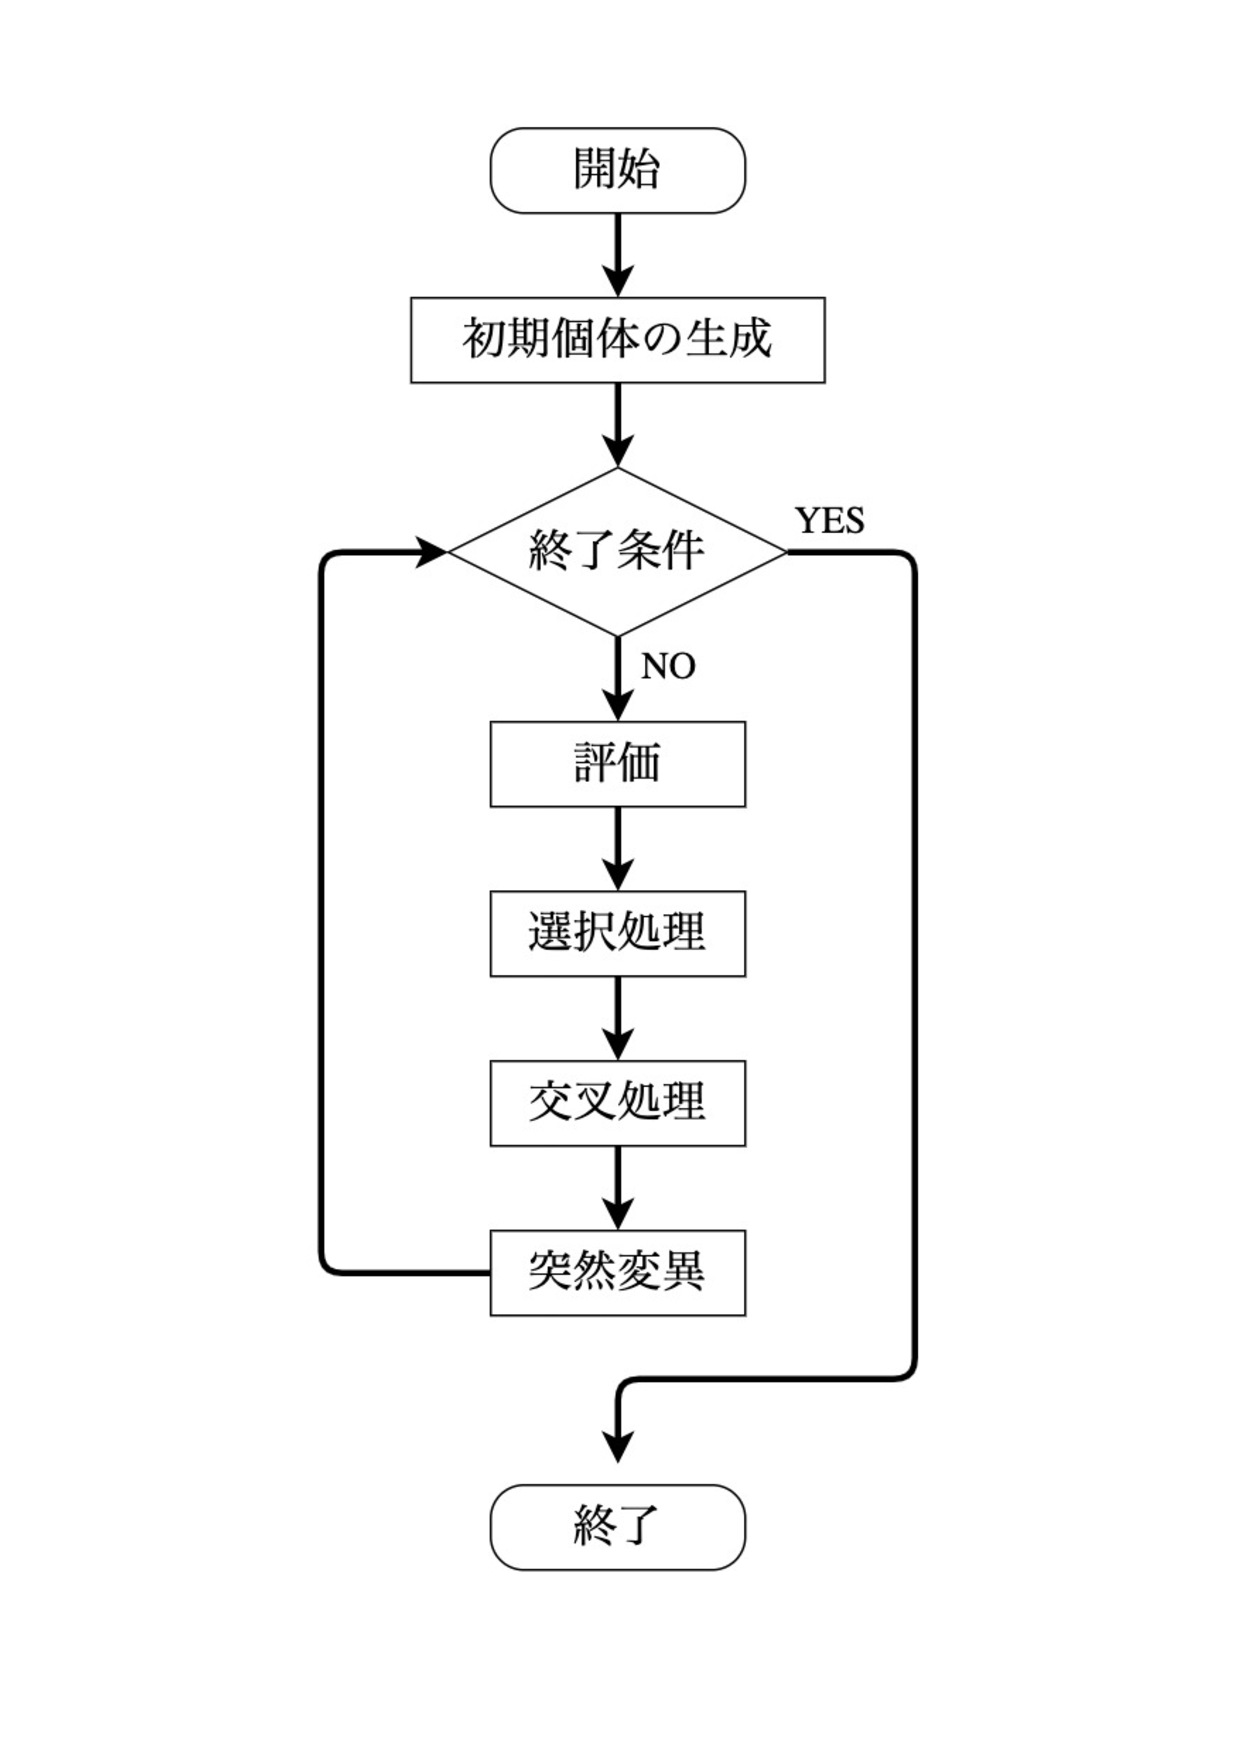
\includegraphics[scale=0.75]{figurefolder/chapter2/GaFlowchart.pdf}
\caption{遺伝的アルゴリズムのフローチャート}
\label{遺伝的アルゴリズムのフローチャート}

\end{center}
\end{figure}

\clearpage


\subsection{各個体の評価処理}
\label{sec2.1.2}
  
各個体の評価処理は,あらかじめ定めた適応度により,各個体の適応度を求める操作である.本処理は遺伝子型と設定されている記号列を実際の評価型にデコーディングして,その表現型と設定されている環境との適応を判定することによって行われる.個体間の適応度の差が激しい場合,選択処理時に適応度の高い個体が選ばれる確率が非常に高くなる.その個体の遺伝子が集団内に増加することにより短時間で探索が収束してしまうため,より適応度の高い遺伝子の探索が困難となる.そこで,適応度の値を直接反映させるのではなく,関数を用いて変換してから,選択に反映させるスケーリングを行う.スケーリング関数の例を示す.表2.1において$f$は元の適応度,$f'$は新たな適応度である.べき乗スケーリングにおいて,$k$はスケーリング指数と呼ばれる.また,シグマ切断の関数において,$\sigma$は適応度の標準偏差,$\bar{f}$は適応度の平均値である.



\begin{table}[!ht]
\caption{スケーリング関数の例}
\label{tb:sk}
\begin{center}
\begin{tabular}{|c||c|}\hline
スケーリング & 関数 \\ \hline
線形スケーリング & $f'=af+b$ \\ \hline
べき乗スケーリング & $f'=f^{k}$ \\ \hline
シグマ切断 & $f'=f-( \bar{f} - c \times \sigma )$ \\ \hline
\end{tabular}
\end{center}
\end{table}

\newpage


\subsection{選択処理}
\label{sec2.1.3}

各個体の選択処理は,集団内での適応度の分布にしたがって,交叉を行う個体の生存分布を決定する操作である.以下に,基本的な選択処理方法である適応度比例方式とエリート保存方式について述べる.

\begin{description}
\item[ (1) ]適応度比例方式

適応度比例方式はルーレット選択方式とも呼ばれ,各個体の子孫がその適応度に比例した確率で選択される方法である.適応度比例方式の最も簡単な実現方法は,適応度に基づいた円グラフをルーレットとして回し,ルーレットの玉が入った領域の個体を選び出すというものである.式(\ref{eq:2.1})に重み付けルーレット方式の式を示す.



\begin{equation}
\vspace{1.0cm}
{p_i}=\frac{f_i}{\displaystyle\sum_{i=1}^{n}f_i}
\label{eq:2.1}
\vspace{-0.5cm}
\end{equation}
式(\ref{eq:2.1})において,$p_i$は$i$番目の個体が親として選ばれる確率,$f_i$は$i$番目の個体適応度,$n$は個体数である.

\item[ (2) ]エリート保存方式

エリート保存方式は,個体の中で最も適応度の高い個体はそのまま次世代に残すという方法である.最も適応度の高い個体は交叉や突然変異による変形を受けないという利点がある.ただし場合によってはあまり良くない遺伝子が急速に集団中に広がる.つまり局所的最適解に収束する危険性がある.そのため一般的には他の選択方法と組み合わせて用いられる.

\end{description}

\newpage

\subsection{交叉処理}
\label{sec2.1.4}

交叉処理は,2つの染色体間で,遺伝子を組み替えて,新たな個体を発生させる操作である.交叉処理で用いられる基本的な手法である一点交叉,複数点交叉,一様交叉について遺伝子列がビット列である場合の例を図に示す.



\begin{description}
\item[ (1) ]一点交叉

図に示すように,遺伝子上に交叉位置をランダムで一点決定する.交叉位置で,親1と親2の遺伝子を入れ替え,子1と子2を発生させる.


\item[ (2) ]複数点交叉

図に示すように,遺伝子上に複数の交叉位置を作る.交叉位置ごとに親1と親2の遺伝子を入れ替え,子1と子2を発生させる.

\item[ (3) ]一様交叉

図に示すように,マスクパターンをランダムに生成する.そして,2つの親個体に対し,そのマスクのビットが0であるなら親1を,1であるなら親2の遺伝子をコピーして子1を発生させる.同時に逆のコピーを行い,子2を発生させる.

\end{description}

\newpage

\begin{figure}[p]
\begin{center}


\subfigure[一点交叉]{
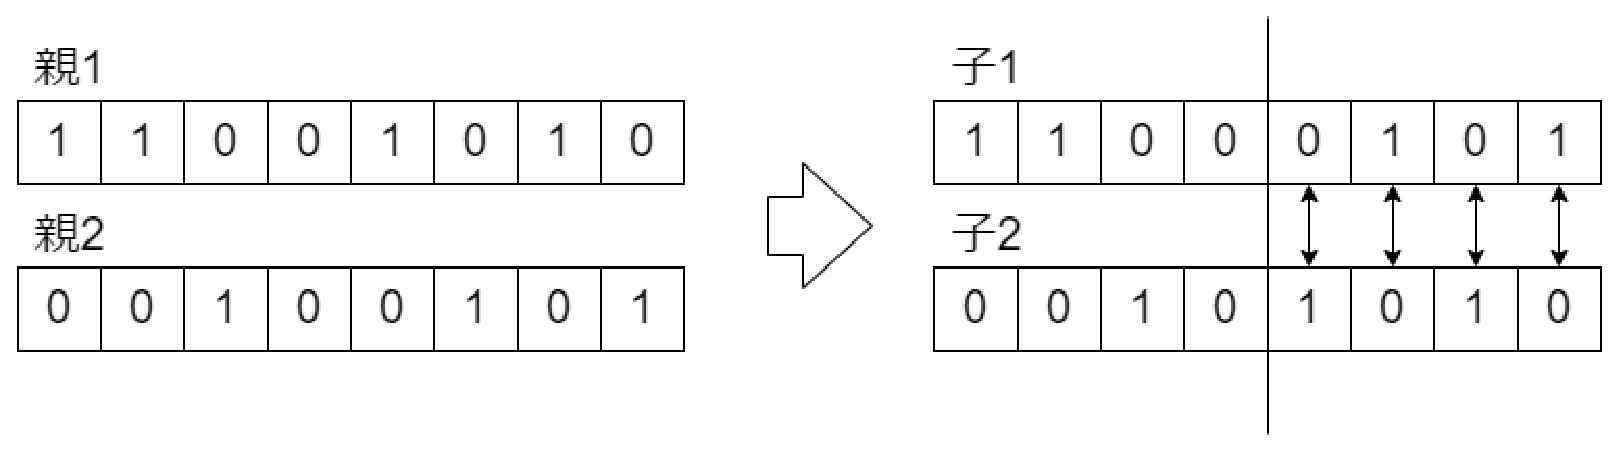
\includegraphics[width=15cm]{figure/chapter2/crossover_1.eps}
\label{一点交叉}}

\subfigure[複数点交叉]{
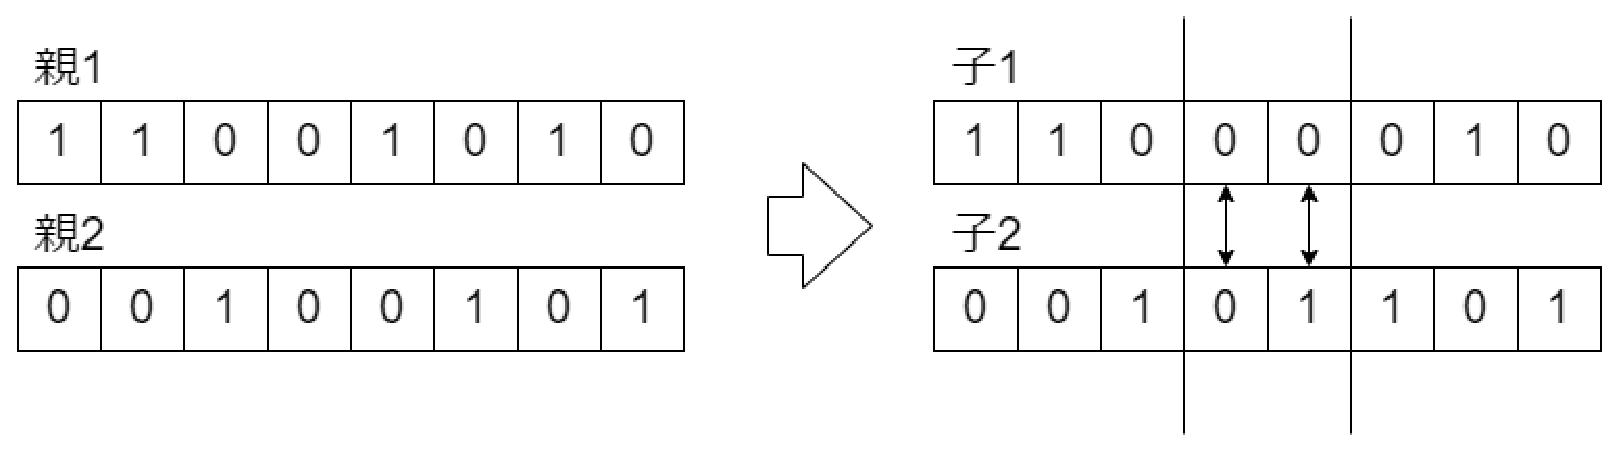
\includegraphics[width=15cm]{figure/chapter2/crossover_2.eps}
\label{複数点交叉}}

\subfigure[一様交叉]{
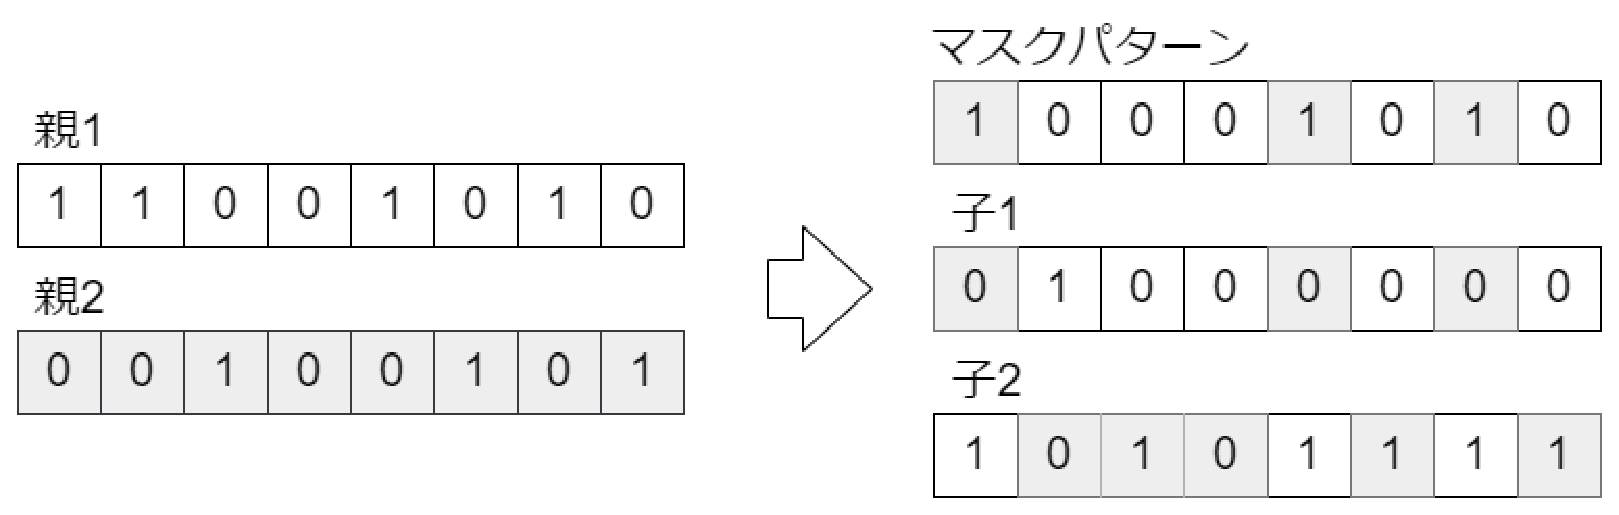
\includegraphics[width=15cm]{figure/chapter2/crossover_3.eps}
\label{一様交叉}}

\caption{交叉処理}
\label{tb:cross}


\end{center}

\end{figure}



\clearpage



\subsection{突然変異処理}
\label{sec2.1.5}

突然変異処理は,遺伝子のある部分を特定の確率で強制的に変化させる操作である.この操作により遺伝子集団に多様性をもたせることでより良い解を持つ個体の発生を促す.ただし,突然変異の確率を大きくしすぎると解の収束が遅くなる.

\begin{description}

\item[ (1) ]転座方式

図に転座方式を示す.転座方式は,遺伝子の一部が同じ遺伝子の他の部分,または他の遺伝子上に位置を移す処理である.

\item[ (2) ]逆位方式


図に逆位方式を示す.逆位方式は,部分的に遺伝子の配列順序を入れ替える処理である.


\end{description}

\begin{figure}[hbt]
\centering
\subfigure[転座方式]{
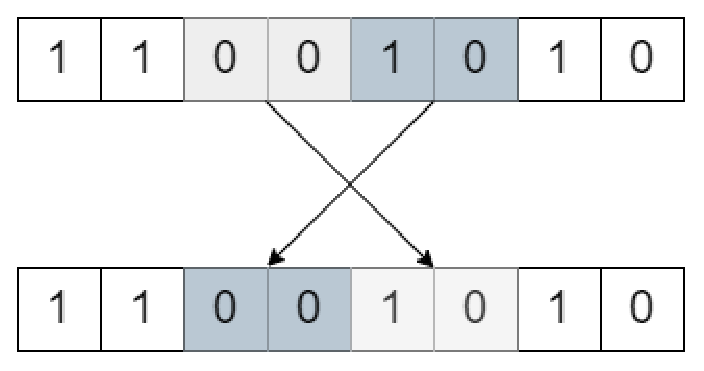
\includegraphics[scale=0.8]{figure/chapter2/mutation_1.eps}
\label{転座方式}}


\subfigure[逆位方式]{
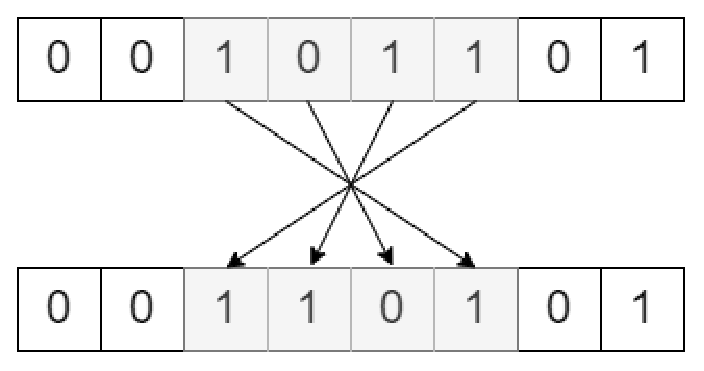
\includegraphics[scale=0.8]{figure/chapter2/mutation_2.eps}
\label{逆位方式}}

\caption{突然変異処理}
\label{fig:2.3}
\end{figure}


\newpage

\section{対話型進化計算}
\label{sec2.2}

\subsection{対話型進化計算の概要}
\label{sec2.2.1}

感性情報を扱うまでは情報処理におけるシステムの最適化は,望ましい出力パラメータを調節することであった.ほとんどの場合,システムの望ましい出力は定量的なものであり,主に誤差最小化規範などを代表とする各種最適化手法が開発されてきた.

しかし近年では,情報処理におけるシステムの最適化の対象は感性情報にまで及んでいる.その場合,望ましい出力がユーザが好む音楽や画像などユーザ自身が主観的に決めるものであるため,望ましい出力を数値的に導くことは困難である.このようなシステムの最適化において,従来と異なる最適化手法が必要となる.その方法の一つとして,ユーザの評価系の代替モデルを作成し,これを従来の最適化システムに組み込むことで数値的に導き出せるようにすることが考えられる.しかし,個人の主観や好みに依存する情報に対応できる正確な代替モデルを構築することは非常に難しい.そこで,ユーザ自身が最適化系に組み込み,ユーザ本人の評価に基づいてコンピュータに最適化させる方法が考えられる.このようにユーザとコンピュータがコミュニケーションをとり,ユーザの主観的評価に基づいて最適化を行う手法のうち,ECを用いる手法をIECと呼ぶ.IECは人間の主観的評価に基づいて最適化を行うため,感性を具現化する技術といえる.

代表的なEC 技術として,GA,タブーサーチ法(Taboo Serch: TS),遺伝的プログラミング (Genetic Programming: GP),進化戦略 (Evolution Strategy: ES),進化的プログラミング (Evolutionary Programming: EP),粒子群最適化 (Particle Swarm Optimization: PSO) などがある.
    
\subsection{対話型遺伝的アルゴリズム}
\label{sec2.2.2}

本研究では,GAにおける評価系に人の感性を組み込んだ手法であるIGAを用いる.
IGAは,GA処理における解候補評価をユーザが自らの感性に基づいて行い,解候補を最適化する手法である.

IGAの基本的な処理の流れを図に示す.まず初期解候補を生成する.次に,解候補をユーザに提示し,ユーザが主観的評価を行う.ユーザによる評価が終了すると,ユーザによって与えられた各解候補の評価をもとに選択・交叉・突然変異等の処理が行われ,新たな解候補を生成し,再びユーザに提示する.このような処理を繰り返し,ユーザの感性に合う解候補を生成する.

IGAは,ユーザ評価を取り入れた進化計算手法であるIECにおいてGAの進化計算アルゴリズムを適応させた手法である.すなわち,IGAとは通常のGAにおいて適応度を決定する処理をユーザが行う手法である.ユーザの主観的評価が適応度に反映されるため,IGAは特にユーザの感覚的,直観的な評価が必要とされる問題の解決に多く用いられる.また一般的にIGAはユーザの評価回数が多いほど最適化性能が高くなる傾向にある.したがって,IGAを用いた最適化システムが十分な最適化性能を発揮するためには多くのユーザ評価が必要となる.しかし,ユーザに多くの評価を求めることは,ユーザの評価負担の増加に繋がる可能性がある.

\begin{figure}[p]
\begin{center}

\vspace{1.5cm}
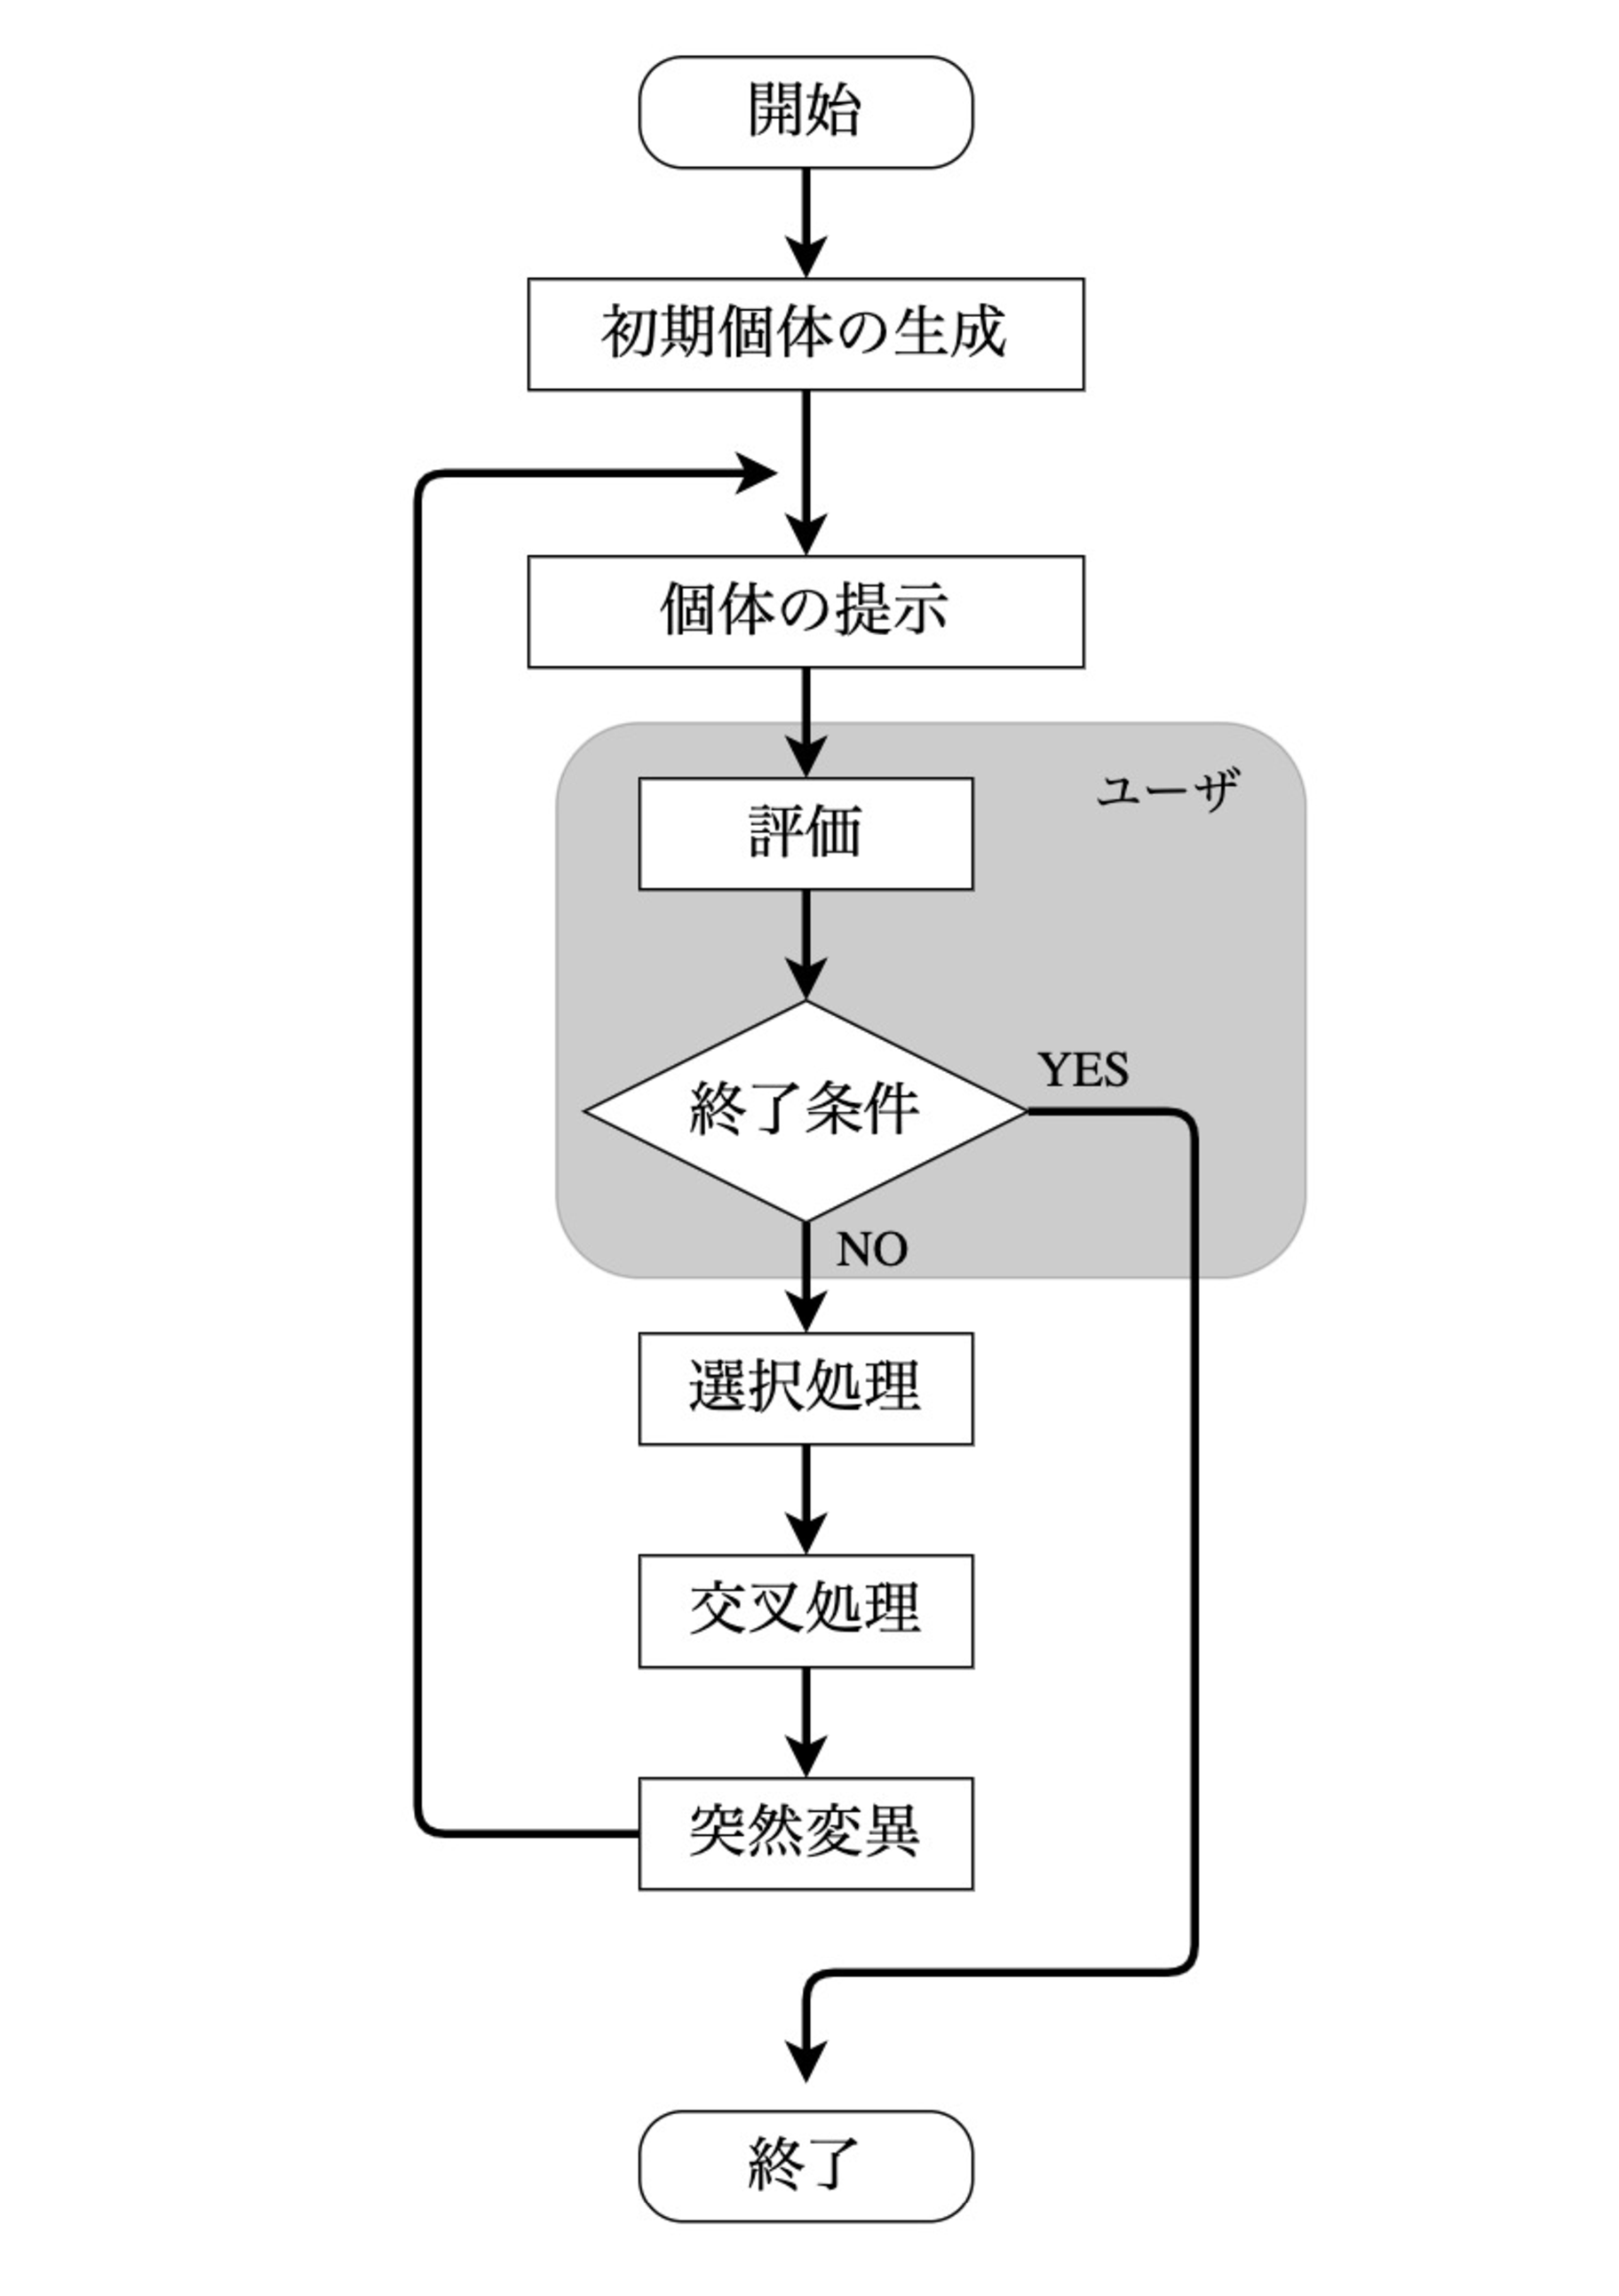
\includegraphics[scale=0.45]{figurefolder/chapter2/IGaFlowchart.pdf}
\caption{遺伝的アルゴリズムのフローチャート}
\label{遺伝的アルゴリズムのフローチャート}

\end{center}
\end{figure}



\newpage

\section{感性とロボット}
\label{sec2.3}

\subsection{ロボットの進化}
\label{sec2.3.1}
近年,ロボット技術の進歩は著しい.人間の代わりに工場などで様々な作業の自動化を行う産業用ロボットは.1960年代に初めて実用化され,普及し始めた.この時代のロボットは,ただ同じ作業を繰り返すだけの作業の代替をするだけであったが,ロボット技術の進歩により様々なロボットが登場した.ロボットはAI,センサ,アームなどの技術進歩によって従来よりも複雑な作業をこなせるようになった.従来の産業用ロボットは比較的大型であり,人との協働作業には不向きであったが,近年では人と協働作業をすることを前提として開発された協働ロボットが実用化されている.
現在では産業用ロボットだけでなく,非産業ロボットであるサービスロボットが普及している.サービスロボットには医療用ロボット,案内ロボット,コミュニケーションロボットなどがある.コミュニケーションロボットには認知所の予防や癒し効果などが期待でき,今後普及が進むと予想されている.


\subsection{性格特性とハンドジェスチャ}
\label{sec2.3.2}
人間らしいコミュニケーションロボットを実現するためには,ロボットの性格特性をジェスチャなどを用いて表現することが重要であるとされている[][].ハンドジェスチャには言葉を強調したり,意味を補完する効果がある[].個人の性格を測る指標としてBig-5理論がよく用いられる.Big-5理論とは,心理学における人の性格は突き詰めると5つの要素の組み合わせからなるとした理論である.Big-5理論における性格特性は,「Openness(開放性)」,「Conscientiousness(誠実性)」,「Extraversion(外向性)」,「Agreauleness(協調性)」,「Neuroticism(神経症的傾向)」から構成される.
Big-5理論は心理学のみならず様々な分野で活用されている.対話中の動作から性格特性を推測する研究[][]や,性格特性からエージェントジェスチャを生成する研究[]などがある.性格特性とハンドジェスチャに関して多くの先行研究がある.ハンドジェスチャは性格特性を表現する重要な指標であることが示されている[][][].
また,性格特性を構成する要素である外向性とハンドジェスチャの関連性について特に多くの研究がされており,外向性の値とハンドジェスチャのスピードや大きさが正の相関があることが示されている[].
また,外向性の値とハンドジェスチャの表出頻度も正の相関があることが示されている[].






\vspace{1cm}
\begin{figure}[!h]
 \begin{center}
  \centering
  \label{fig:kansei}
 \end{center}
\end{figure}



% !TEX root = MasterPaper.tex
\chapter{臨場感を演出する集団ロボットの内部モデル}
\thispagestyle{fancy} % このページのみ
\lhead{}
\chead{}
\rhead{}
\lfoot{} 
\cfoot{\thepage}  
\rfoot{}
%

\section{モデルの概要}
\label{sec3.1}

本研究では,ユーザは感情表出を行うロボット集団と共に野球観戦を行う.その中で,提案ロボット集団はユーザへの感情伝播を行い,観戦時特有の臨場感を演出することを目的とする.

本節では,野球観戦するロボットが試合状況を読み取って感情表出するための内部モデルを紹介する.初めに試合状況を読み取る方法について,次にロボットの表出する感情の生成方法について述べる.

\subsection{試合状況の読み取り}
\label{sec3.1.1}    

本研究では,ロボットは観戦する試合状況を読み取ることで,試合展開に沿った感情表出を行う.試合状況は,プロ野球情報サイトである「キューステ!」で利用されている「勝利確率グラフ」を用いて読み取る\cite{kyusute}.ここで,勝利確率グラフとは,特定の試合状況(イニング・点差・走者・アウトカウント)において,チームにどれだけ勝利が見込まれるかをグラフ化したものである.

勝利確率グラフで示される値である勝利確率$Q$は,過去のチームの勝利数$S$と過去の同じ状況の場面数$N$を用いて式(\ref{eq:3.1})のように算出する.勝利数$S$と場面数$N$の値は,1995年~2018年の日本プロ野球公式記録を参照する.2019年4月5日に開催された阪神タイガース-広島東洋カープの試合の勝利確率グラフの例を図\ref{win_percent}に示す.試合開始の時点では両チームにそれぞれ50%の勝利確率が見込まれ,回が進み点差が開くほど優位なチームは100%に近付いていく.また,得点期待の高いシーンや,終盤の勝敗に直結するシーンなどは勝利確率が大きく変動する.

\vspace{1cm}
 \begin{figure}[H]
 \begin{center}
  \centering
  \includegraphics[width=13.5cm]{images/chapter3/winper.eps}
  \caption{勝利確率グラフ}
  \label{win_percent}
 \end{center}
\end{figure}


\begin{equation}
\label{eq:3.1}
 Q = \frac{S}{N}
\end{equation}





\subsection{感情の生成方法}
\label{sec3.1.2}

先行研究では,野球観戦において得点に対する期待感が高まる場面で,観戦者の歓声量が増加することが分かっている\cite{rinjyo3}.つまり,観戦者は勝利の確率が変動する場面で,感情を表出しているといえる.そのため,ロボットが観戦者と同じような場面で感情表出を行うことで,ユーザはロボットと違和感なく野球観戦をすることができると考えられる.

そこで,本研究では,ロボットは勝利確率グラフの増減値の幅$W$を用いて感情の生成を行う.増減値の幅$W$は現在の勝利確率$Q_{a}$と1つ前の勝利確率$Q_{b}$を用いて式(\ref{eq:3.2})のように定義する.
\begin{equation}
\label{eq:3.2}
 W = \frac{Q_{a}-Q_{b}}{100}
\end{equation}

現在のシーンの勝利確率を$Q_{a}$,1つ前のシーンの勝利確率を$Q_{b}$とし,100で割ることによって勝利確率の増減値の幅を算出する.

提案するロボットは,喜の感情と哀の感情の2種類の感情を生成する.$W$の符号によって感情の種類を決定し,$W > 0$なら喜の感情を,$W < 0$なら哀の感情を表出する.


\newpage

\section{実験環境}
\label{sec3.2}

実環境でのインタラクションにおいて,感情を表出するロボット集団を準備することや,リアルタイムでの勝利確率を取得することは困難であるため,本実験では仮想環境であるVR空間を用いて実験を行う.本研究では,採用しているバーチャルアバターをロボットと呼ぶ.ロボット集団と共に野球観戦を行うため,スポーツバーを模した空間をゲームエンジンであるUnityを用いて制作している\cite{unity}.

本実験では,観戦を行う場所としてスポーツバーを模した内装と,感情を表出するロボット集団を,Unity内のAsset storeにある有償のAssetを改変して使用している\cite{bar}\cite{lilrobot}.スポーツバーとロボット集団の外観を図\ref{sports_bar},図\ref{robot}に示す.

また,Unityで作成したVR空間を体験するためのデバイスとして,ヘッドマウントディスプレイ,ヘッドフォンを使用する.この機器は家庭用VRデバイスであるHTC VIVEを用いる\cite{vive}.

本実験で使用するヘッドフォン付きヘッドマウントディスプレイを図\ref{Vive}に示す.


\vspace{1cm}
 \begin{figure}[H]
 \begin{center}
  \centering
  \includegraphics[width=15cm]{images/chapter3/sports_bar.eps}
  \caption{実験環境}
  \label{sports_bar}
 \end{center}
\end{figure}


\newpage

\vspace{1cm}
 \begin{figure}[!h]
 \begin{center}
  \centering
  \includegraphics[width=15cm]{images/chapter3/robot.eps}
  \caption{ロボット集団}
  \label{robot}
 \end{center}
\end{figure}


\vspace{1cm}
 \begin{figure}[!h]
 \begin{center}
  \centering
  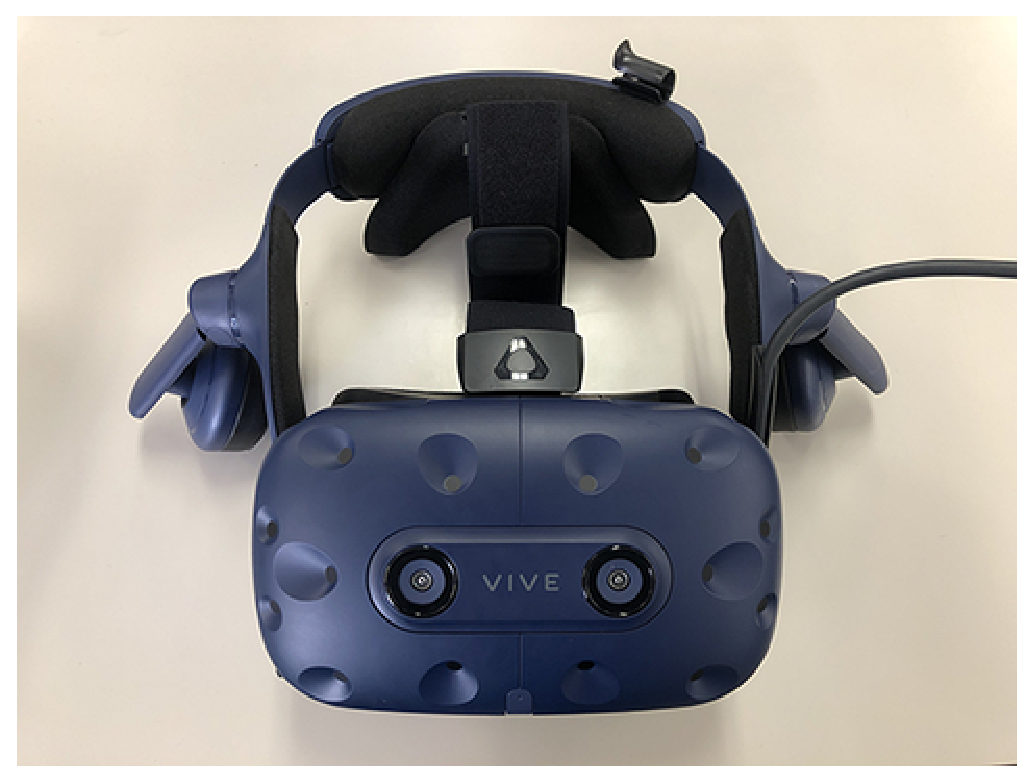
\includegraphics[width=12cm]{images/chapter3/Vive.eps}
  \caption{ヘッドマウントディスプレイ}
  \label{Vive}
 \end{center}
\end{figure}


\subsection{スポーツバーでの観戦}
\label{sec3.2.1}

実験中の画面の様子を図\ref{bar_scene}に示す.本実験では被験者とロボットのみで試合観戦を行う.共に試合観戦を行うロボット集団は,スポーツバーを模した空間上の席に着席して試合観戦を行う.

被験者はヘッドフォン付きヘッドマウントディスプレイを装着して着席し,その場から動かずにロボット集団と試合観戦を行う.図\ref{sports_bar}の前方にある4台のモニターに映し出される試合を観戦する.また,ヘッドマウントディスプレイによる映像だけでなく,ヘッドフォンからは観戦映像の音が流れている.このように,被験者は視覚情報と聴覚情報の2つを用いて試合観戦を行う.




\vspace{1cm}
 \begin{figure}[!h]
 \begin{center}
  \centering
  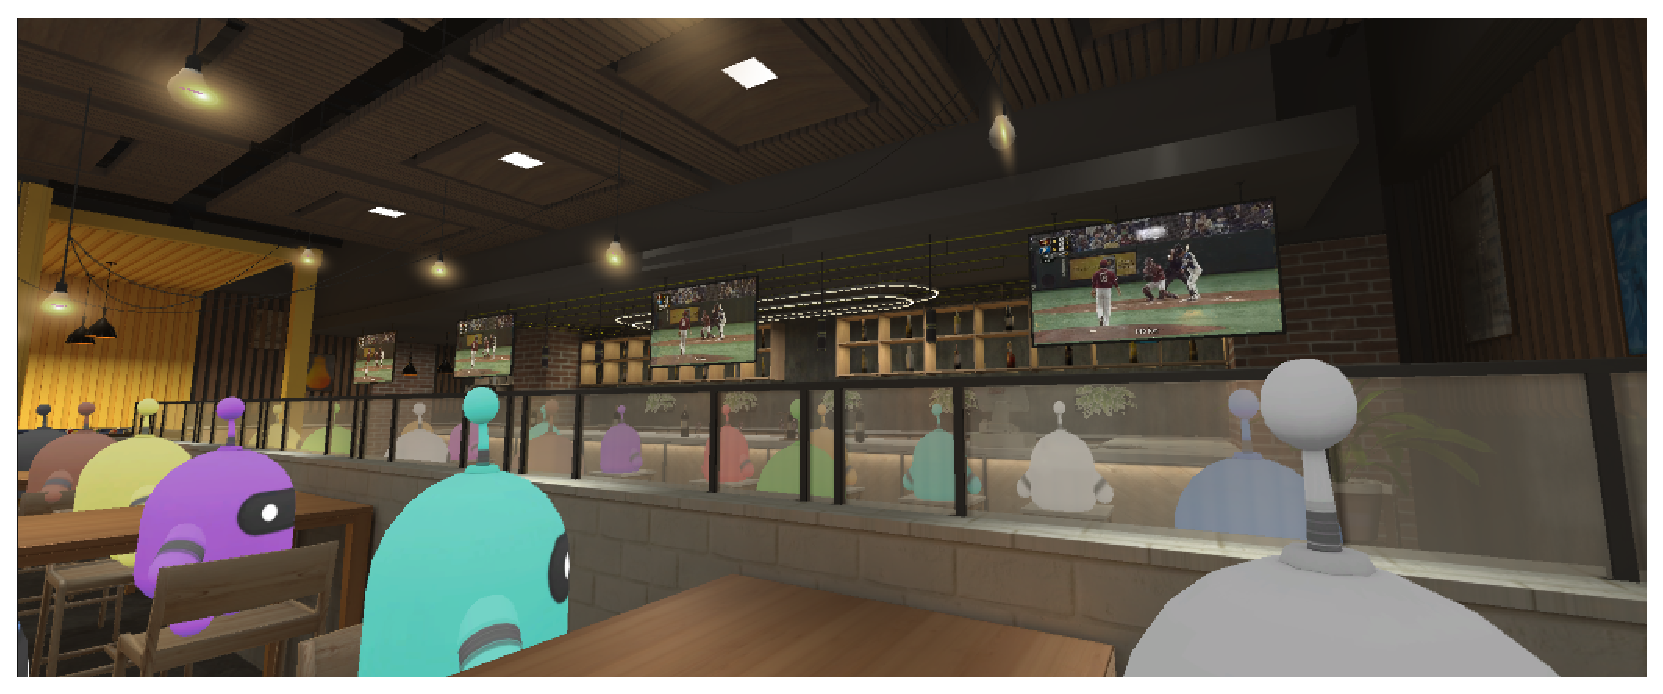
\includegraphics[width=15cm]{images/chapter3/bar_scene.eps}
  \caption{スポーツバーの様子}
  \label{bar_scene}
 \end{center}
\end{figure}



\newpage



\subsection{ロボット集団の動作}
\label{sec3.2.2}

被験者と共に試合観戦をするロボット集団は,感情表出しない状態(Idle状態),喜の感情表出,哀の感情表出を行う.

Idle状態では,ロボットは図\ref{Idle}の状態から,一定の周期でゆっくりと上下に反復運動を行う.この動作によって,人間の呼吸運動を再現する.また,各ロボットは,反復運動の速さを24回/分,27回/分,30回/分,33回/分,36回/分の5種類からランダムで設定されており,速さを変えることによってロボットの個性を設計している.

喜の感情表出は,図\ref{happy}のように,手を挙げながらジャンプする動作を繰り返すことで表出する.表出する感情の程度は,ジャンプする動作の速さを変更することで設計する.本実験では感情の程度を小,中,大の3種類に設定し,小なら30回/分,中なら50回/分,大なら70回/分の速さで感情表出を行う.

哀の感情表出は,図\ref{sad}のように,飛び上がって倒れこむ動作を繰り返すことで表出する.表出する感情の程度は,倒れこむ速さを変更することで設計する.喜の感情と同じく3段階の感情の程度を設定し,小なら12回/分,中なら15回/分,大なら20回/分の速さで感情表出を行う.


\vspace{1cm}
 \begin{figure}[!h]
 \begin{center}
  \centering
  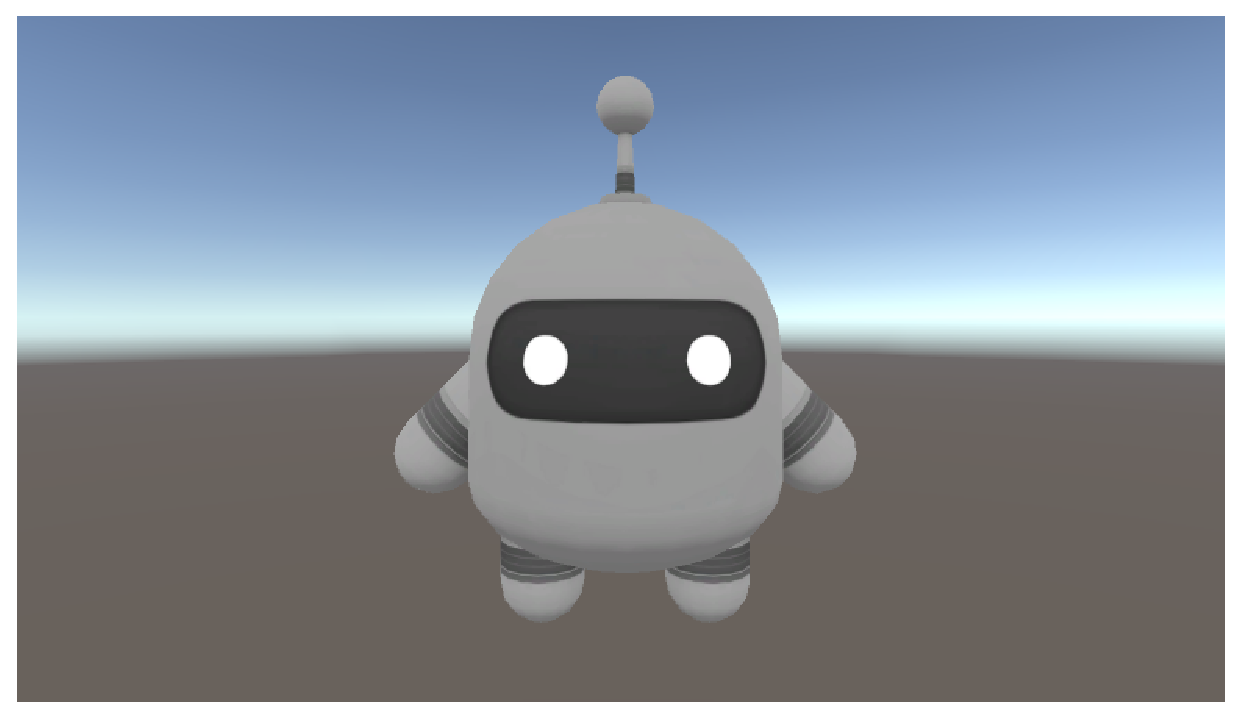
\includegraphics[width=12cm]{images/chapter3/Idle.eps}
  \caption{Idle状態のロボット}
  \label{Idle}
 \end{center}
\end{figure}

\vspace{1cm}
 \begin{figure}[!h]
 \begin{center}
  \centering
  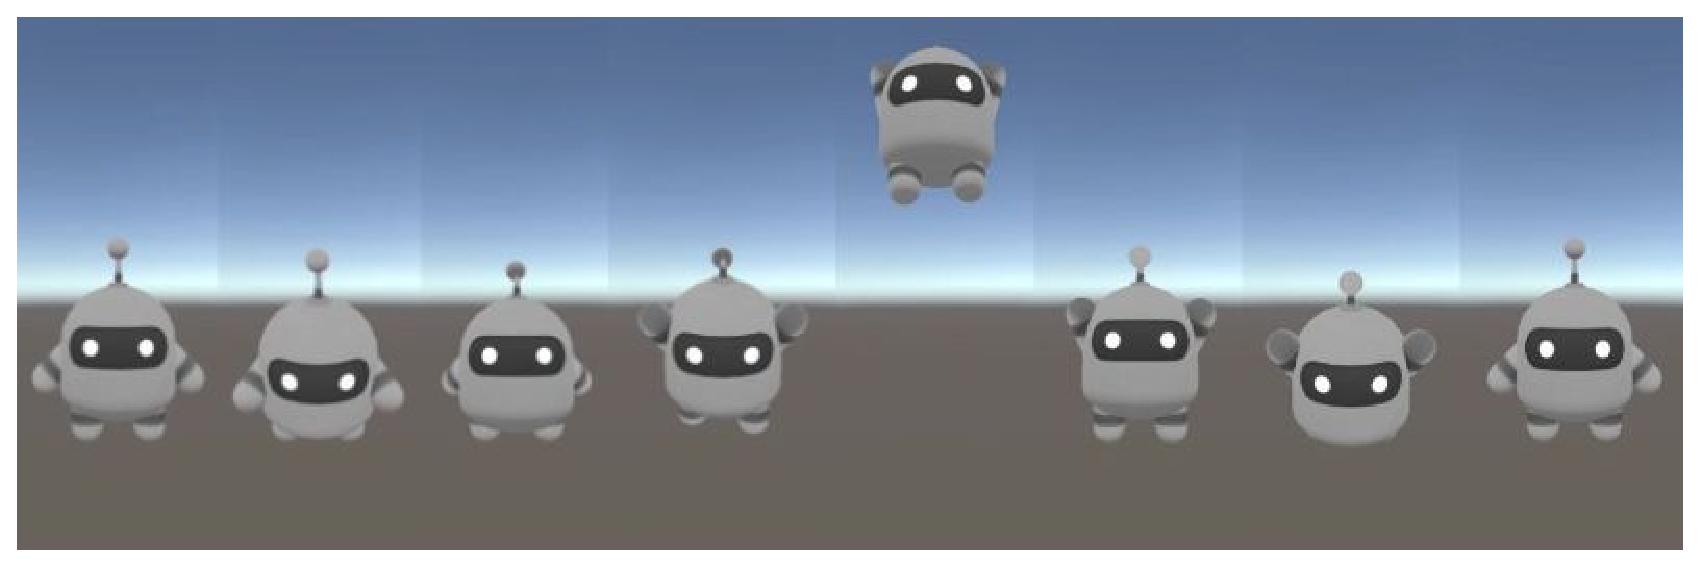
\includegraphics[width=12cm]{images/chapter3/happy.eps}
  \caption{喜の表出感情}
  \label{happy}
 \end{center}
\end{figure}

\vspace{1cm}
 \begin{figure}[!h]
 \begin{center}
  \centering
  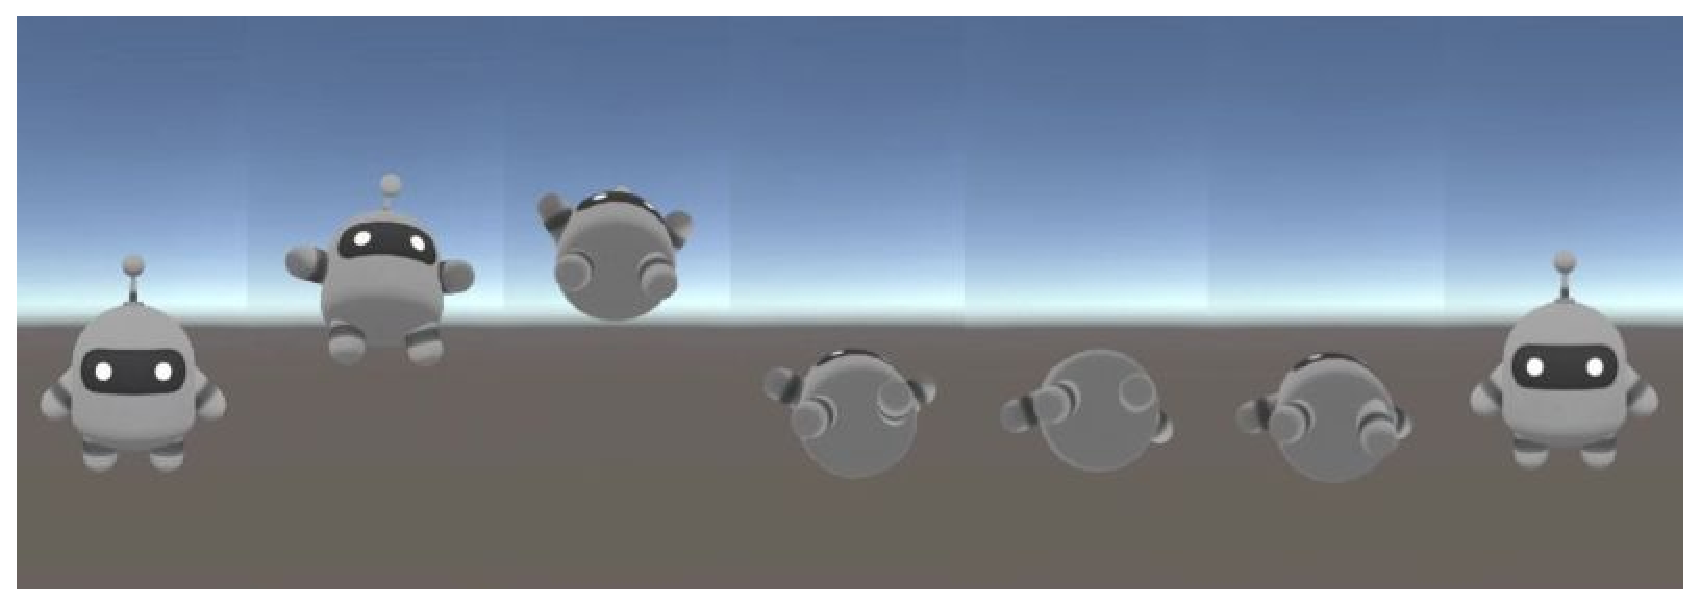
\includegraphics[width=12cm]{images/chapter3/sad.eps}
  \caption{哀の表出感情}
  \label{sad}
 \end{center}
\end{figure}

\newpage




















% !TEX root = MasterPaper.tex
\chapter{実ユーザによる評価実験}
\thispagestyle{fancy}
\lhead{}
\chead{}
\rhead{}
\lfoot{} 
\cfoot{\thepage}  
\rfoot{}
%

\section{実験概要}
\label{sec4.1}

本実験では,被験者にはヘッドマウントディスプレイを装着し,VR空間内のスポーツバーを模した空間で提案ロボット集団,比較ロボット集団と野球観戦を行ってもらう.比較ロボット集団とは感情表出の程度が異なるロボット集団である.感情表出の詳細については4.2.2で述べる.実験前に,被験者に対して本研究で示すスポーツ観戦における臨場感演出の定義について説明する.順序効果を防ぐため,被験者を提案ロボット集団,比較ロボット集団の順に観戦を行うグループと,比較ロボット集団,提案ロボット集団の順に観戦を行うグループに分ける.ロボット集団の総数は34体であり,被験者と同じチームを応援するロボットが22体,被験者と異なるチームを応援するロボットが12体になっている.ロボット集団の印象に関するアンケートは各ロボット集団との観戦後に回答してもらう.また,各ロボット集団の比較に関するアンケートは実験終了後に回答してもらう.

本実験の被験者は野球観戦に興味がある,また野球に関する知識がある20代の男女12名である.

ロボット集団の印象に関するアンケート項目を表\ref{question1}に示す.表\ref{question1}の計8つの質問に加えて自由記述からなるアンケートである.本アンケートはそれぞれ「そう思う/少しそう思う/どちらでもない/あまりそう思わない/そう思わない」の5段階で評価する.

Q1は,ロボット集団の感情表出によって観戦の楽しさに差が生まれるかを調査するための質問である.Q2~Q5は,ロボット集団との観戦で臨場感を演出することができるかを問う質問である.Q6~Q8はロボット集団への親和性を問う質問である.

次に,ロボット集団の比較に関するアンケート項目を表\ref{question2}に示す.表\ref{question2}の計7つの質問に加えて自由記述からなるアンケートである.本アンケートはそれぞれ「1回目のロボット集団/どちらかといえば1回目のロボット集団/どちらともいえない/どちらかといえば2回目のロボット集団/2回目のロボット集団」の5段階で評価する.

Q9は,ロボット集団の感情表出によって観戦の楽しさにどのくらいの差が生まれるかを調査するための質問である.Q10~Q12は,ロボット集団との観戦における臨場感演出の差を調査する質問である.Q13~Q15は,ロボット集団の親和性の差を調査する質問である.


\begin{table}[!ht]
\caption{ロボット集団の印象に関するアンケート項目}
\label{question1}
\begin{center}
\begin{tabular}{|l||l|}\hline
Q1&ロボット集団との観戦を楽しむことができたか\\ \hline
Q2&実際にロボット集団は観戦しているように感じたか\\ \hline
Q3&ロボット集団との観戦で一体感を感じることができたか\\ \hline
Q4&ロボット集団との観戦で臨場感を感じることができたか\\ \hline
Q5&ロボット集団の感情表出に感化されたか\\ \hline
Q6&ロボット集団に人間らしさを感じたか\\ \hline
Q7&ロボット集団に親しみを持てたか\\ \hline
Q8&またこのロボット集団と一緒に観戦したいか\\ \hline

\end{tabular}
\end{center}
\end{table} 

\begin{table}[!ht]
\caption{ロボット集団の比較に関するアンケート項目}
\label{question2}
\begin{center}
\begin{tabular}{|l||l|}\hline
Q9&どちらのロボット集団との観戦が楽しかったか\\ \hline
Q10&どちらのロボット集団に一体感を感じたか\\ \hline
Q11&どちらのロボット集団に臨場感を感じたか\\ \hline
Q12&どちらのロボット集団の感情表出に感化されたか\\ \hline
Q13&どちらのロボット集団に人間らしさを感じたか\\ \hline
Q14&どちらのロボット集団に親しみを持てたか\\ \hline
Q15&どちらのロボット集団とまた一緒に観戦したいか\\ \hline

\end{tabular}
\end{center}
\end{table} 

\clearpage

\section{実験条件}
\label{sec4.2}

\subsection{観戦する試合映像}
\label{sec4.2.1}

本実験では,被験者の疲労を考慮して,野球中継を8分程度にまとめたハイライト形式の映像を被験者に観戦してもらう.ハイライトは,日本プロ野球のパシフィック・リーグの試合を動画配信するインターネットテレビサービスである「パ・リーグTV」で提供されているアーカイブ動画を使用する\cite{patv}.
このアーカイブ動画を8分程度にまとめるため,試合内で勝利確率の増減値の幅$W$が$|W|\geq0.05$のシーンを切り抜き,繋げることで作成する.

本実験では,2021年4月16日に開催された北海道日本ハムファイターズ-東北楽天ゴールデンイーグルスの第4回戦と,同年4月18日に開催された同チームの第6回戦を用いて実験を行う.どちらも1-4で東北楽天ゴールデンイーグルスが勝利しており,試合展開は似通ったものになっている.2試合の勝利確率グラフを図\ref{0416},図\ref{0418}に示す.また,被験者には勝利チームを応援してもらう.




\subsection{ロボット集団のパラメータ}
\label{sec4.2.2}

提案ロボットと比較ロボットは感情表出のしやすさが異なる.

ロボットの感情表出の条件は以下のようになっており,式(\ref{eq:4.1})なら小の感情を,式(\ref{eq:4.2})なら中の感情を,式(\ref{eq:4.3})なら大の感情を表出する.
\begin{equation}
\label{eq:4.1}
 x \leq |W| \leq x + a
\end{equation}
\begin{equation}
\label{eq:4.2}
 x + a \leq |W| \leq x + 2a
\end{equation}
\begin{equation}
\label{eq:4.3}
 x + 2a \leq |W| 
\end{equation}


$W$は勝利確率の増減値の幅であり,$x$は各ロボットの感情表出のしやすさを表すパラメータである.また,$a$は感情の程度のパラメータである.$a$はハイライトに用いたシーンの増減値の平均値より決定しており,本実験では$a = 0.05$としている.

提案ロボットは,感情表出しやすいロボットである.提案ロボットが持つ,感情表出のしやすさを表すパラメータ$x$は,
$0.01 \leq x \leq 0.05$の範囲でランダムに与えられる.作成したハイライトは$|W| \geq 0.05$のシーンから構成されているため,全てのシーンで,少なくとも小の感情を表出する.

比較ロボットは提案ロボットとは異なり,勝敗が決定するシーン以外では感情表出せず,試合観戦を行うロボットである.比較ロボットのパラメータ$x$は,$0.15 \leq x \leq 0.20$の範囲でランダムに与えられる.このパラメータにより,比較ロボットはほとんどのシーンで感情表出を行わない.

\newpage

\vspace{1cm}
\begin{figure}[!h]
 \begin{center}
  \centering
  \includegraphics[width=13cm]{images/chapter4/0416.eps}
  \caption{2021年4月16日に行われた試合の勝利確率グラフ}
  \label{0416}
 \end{center}
\end{figure}


\vspace{1cm}
\begin{figure}[!h]
 \begin{center}
  \centering
  \includegraphics[width=13cm]{images/chapter4/0418.eps}
  \caption{2021年4月18日に行われた試合の勝利確率グラフ}
  \label{0418}
 \end{center}
\end{figure}


\newpage


\section{実験結果}
\label{sec4.3}

実験後に行うアンケート結果より,提案ロボット集団が被験者に臨場感を与えられたかを検証する.提案ロボット集団と比較ロボット集団への印象に関するアンケート結果を図\ref{Q1}~図\ref{Q8}に示す.また,実験終了後に行ったアンケート結果より,提案ロボット集団と比較ロボット集団を比較して,どのくらい臨場感の演出に差があったかを検証する.提案ロボット集団と比較ロボット集団の比較に関するアンケート結果を図\ref{Q9}~図\ref{Q15}に示す.

まず,ロボット集団の印象について問う質問であるQ1~Q8について述べる.Q1のアンケート結果より,被験者は頻繁に感情を表出する提案ロボット集団との観戦により,観戦時に楽しさが生じたことが分かる.Q2,Q3のアンケート結果より,提案ロボット集団との観戦で,被験者はロボット集団と共に観戦し,一体感を感じていたことが分かる.Q4のアンケート結果では,半数の被験者が提案ロボット集団への質問で「そう思う」「少しそう思う」と回答した.比較ロボット集団への質問では,被験者の大半が「あまりそう思わない」「そう思わない」と回答したことから,概ね臨場感が演出できていたと言える.Q5のアンケート結果より,被験者は提案ロボット集団の動作による感情表出に感化されたことが分かる.Q6,Q7,Q8のアンケート結果より,提案ロボット集団に親和性を感じていたことが分かる.


次に,ロボット集団の比較について問う質問であるQ9~Q15について述べる.Q9のアンケート結果より,91.7%の被験者が提案ロボット集団との観戦の方がより楽しかったと回答した.Q10のアンケート結果より,被験者全員が提案ロボット集団との観戦でより一体感を感じたと回答した.Q11のアンケート結果より,被験者全員が提案ロボット集団との観戦でより臨場感を感じたと回答した.Q12のアンケート結果より,91.7%の被験者が提案ロボット集団の方がより感化されたと回答した.Q13,Q14,Q15のアンケート結果より,提案ロボット集団の方が,より親和性を感じていることが分かる.

アンケートの自由記述欄には,提案ロボット集団について,「実際に人と一緒に観戦しているみたいで楽しかった」「動作だけでも一体となって楽しんでいる感覚があった」という,本実験の目的に沿った記述が多く見られた.また,比較ロボット集団について,「自分が喜んでいる時にロボットが喜んでおらず臨場感を感じることができなかった」といった記述が見られた.こちらも,本実験の目的に沿っていると言える.一方で,ロボット集団の感情表出方法として,歓声による方法や,動作の種類を増やすことによる複雑な表出についてなどの指摘も見られた.


\newpage

\begin{figure}[!h]
 \begin{center}
\vspace{3cm}
  \centering
  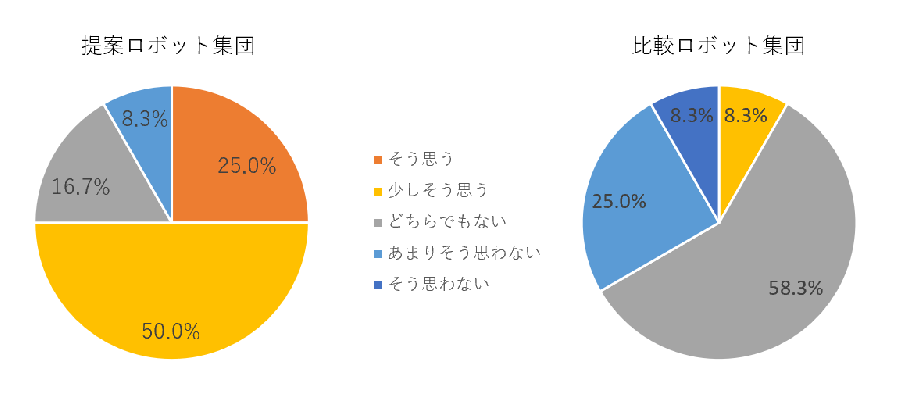
\includegraphics[width=15cm]{images/chapter4/Q1.eps}
  \caption{「ロボット集団との観戦を楽しむことができたか」のアンケート結果}
  \label{Q1}
 \end{center}
\end{figure}



\begin{figure}[!h]
 \begin{center}
\vspace{3cm}
  \centering
  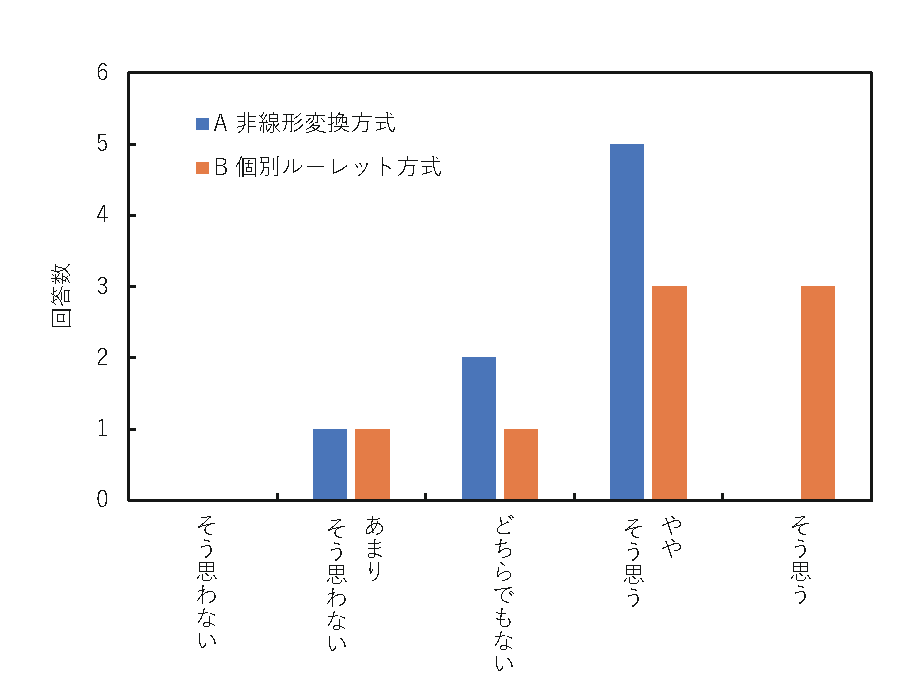
\includegraphics[width=15cm]{images/chapter4/Q2.eps}
  \caption{「実際にロボット集団は観戦しているように感じたか」のアンケート結果}
  \label{Q2}
 \end{center}
\end{figure}



\newpage

\begin{figure}[!h]
 \begin{center}
\vspace{3cm}
  \centering
  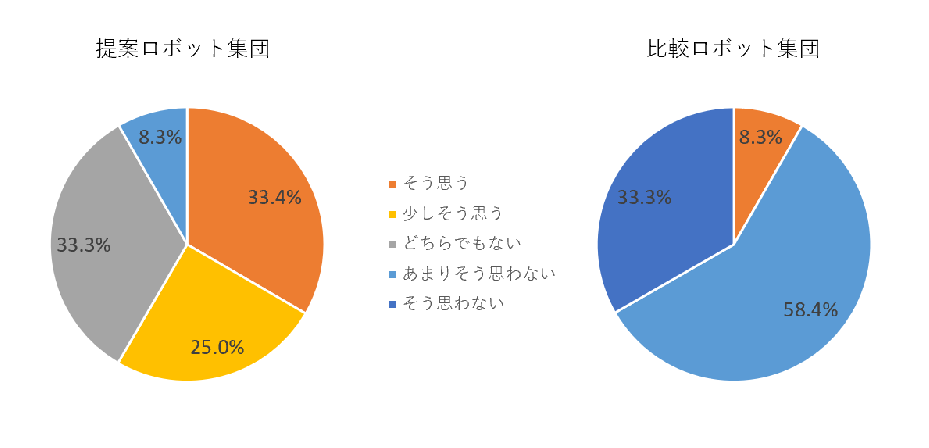
\includegraphics[width=15cm]{images/chapter4/Q3.eps}
  \caption{「ロボット集団との観戦で一体感を感じることができたか」のアンケート結果}
  \label{Q3}
 \end{center}
\end{figure}



\begin{figure}[!h]
 \begin{center}
\vspace{2cm}
  \centering
  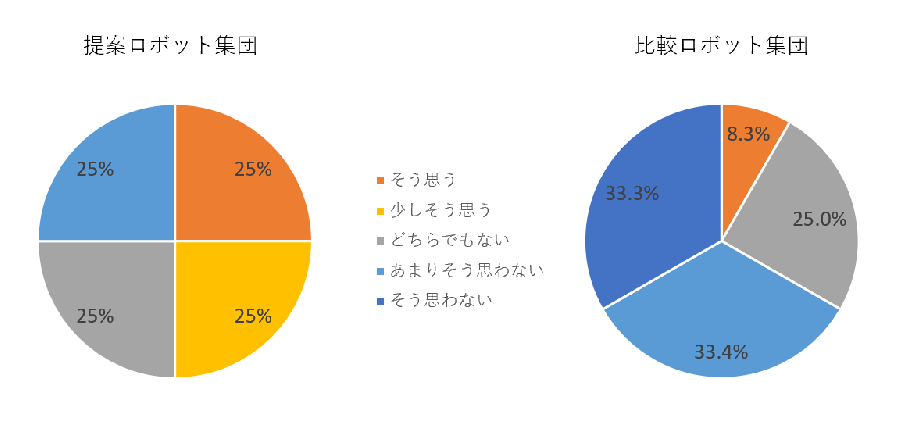
\includegraphics[width=15cm]{images/chapter4/Q4.eps}
  \caption{「ロボット集団との観戦で臨場感を感じることができたか」のアンケート結果}
  \label{Q4}
 \end{center}
\end{figure}

\newpage


\begin{figure}[!h]
 \begin{center}
\vspace{3cm}
  \centering
  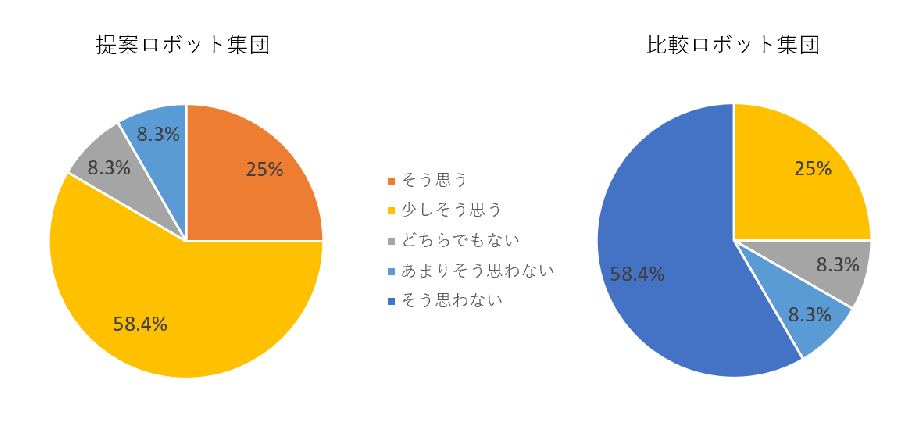
\includegraphics[width=15cm]{images/chapter4/Q5.eps}
  \caption{「ロボット集団の感情表出に感化されたか」のアンケート結果}
  \label{Q5}
 \end{center}
\end{figure}



\begin{figure}[!h]
 \begin{center}
\vspace{3cm}
  \centering
  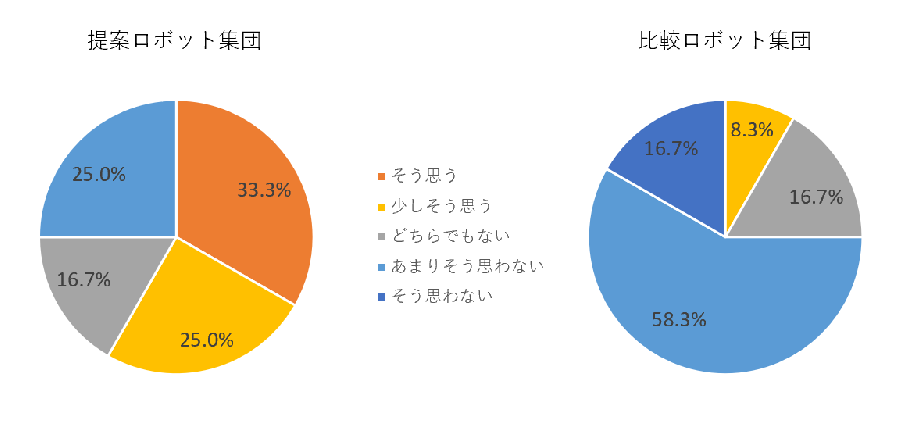
\includegraphics[width=15cm]{images/chapter4/Q6.eps}
  \caption{「ロボット集団に人間らしさを感じたか」のアンケート結果}
  \label{Q6}
 \end{center}
\end{figure}

\newpage



\begin{figure}[!h]
 \begin{center}
\vspace{3cm}
  \centering
  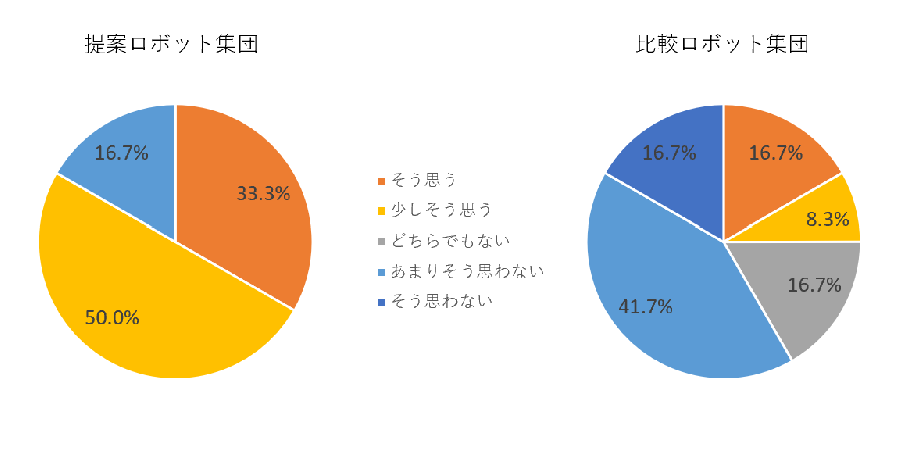
\includegraphics[width=15cm]{images/chapter4/Q7.eps}
  \caption{「ロボット集団に親しみを持てたか」のアンケート結果}
  \label{Q7}
 \end{center}
\end{figure}




\begin{figure}[!h]
 \begin{center}
\vspace{2cm}
  \centering
  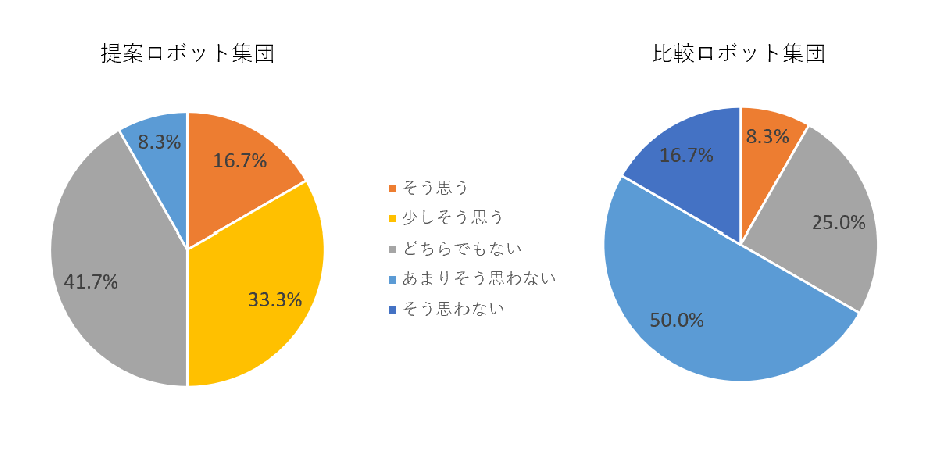
\includegraphics[width=15cm]{images/chapter4/Q8.eps}
  \caption{「またこのロボット集団と一緒に観戦したいか」のアンケート結果}
  \label{Q8}
 \end{center}
\end{figure}



\newpage

\vspace{1cm}
\begin{figure}[!h]
 \begin{center}
  \centering
  \includegraphics[width=15cm]{images/chapter4/Q9.eps}
  \caption{どちらのロボット集団の観戦が楽しかったか}
  \label{Q9}
 \end{center}
\end{figure}

\vspace{1cm}
\begin{figure}[!h]
 \begin{center}
  \centering
  \includegraphics[width=15cm]{images/chapter4/Q10.eps}
  \caption{どちらのロボット集団に一体感を感じたか}
  \label{Q10}
 \end{center}
\end{figure}

\newpage

\vspace{1cm}
\begin{figure}[!h]
 \begin{center}
  \centering
  \includegraphics[width=15cm]{images/chapter4/Q11.eps}
  \caption{どちらのロボット集団に臨場感を感じたか}
  \label{Q11}
 \end{center}
\end{figure}

\vspace{1cm}
\begin{figure}[!h]
 \begin{center}
  \centering
  \includegraphics[width=15cm]{images/chapter4/Q12.eps}
  \caption{どちらのロボット集団の感情表出に感化されたか}
  \label{Q12}
 \end{center}
\end{figure}

\newpage

\vspace{1cm}
\begin{figure}[!h]
 \begin{center}
  \centering
  \includegraphics[width=15cm]{images/chapter4/Q13.eps}
  \caption{どちらのロボット集団に人間らしさを感じたか}
  \label{Q13}
 \end{center}
\end{figure}

\vspace{1cm}
\begin{figure}[!h]
 \begin{center}
  \centering
  \includegraphics[width=15cm]{images/chapter4/Q14.eps}
  \caption{どちらのロボット集団に親しみを持てたか}
  \label{Q14}
 \end{center}
\end{figure}

\newpage

\vspace{1cm}
\begin{figure}[!h]
 \begin{center}
  \centering
  \includegraphics[width=15cm]{images/chapter4/Q15.eps}
  \caption{どちらのロボット集団とまた一緒に観戦したいか}
  \label{Q15}
 \end{center}
\end{figure}





\newpage

\section{考察}
\label{sec4.4}

図\ref{Q1}より,頻繁に感情を表出するロボット集団との観戦で,被験者は楽しさを感じていたことが分かる.これは,実空間での観戦を提案ロボット集団との観戦で再現できていたためだと考えられる.また,図\ref{Q2}~図\ref{Q5}より,被験者は提案ロボット集団との観戦で,本研究で示している臨場感の構成要素である,没入感や一体感,ロボット集団からの感情伝播に関する評価が高かったことが分かる.一方で,臨場感そのものについて問う質問では,半数の被験者がどちらでもない,あるいは低評価だと回答しており,十分な結果とは言えなかった.この結果から,没入感や一体感,感情伝播以外にも,スポーツ観戦において,臨場感を演出するために必要な要素があると考えられる.

両ロボットを比較する質問である図\ref{Q9}~図\ref{Q15}より,被験者の9割以上が,提案ロボット集団の方が,共に試合観戦を行うロボット集団に適していると感じていたことが分かる.この結果から,スポーツ観戦において臨場感を演出するためには,周囲の感情表出が必要不可欠であると考えられる.一方で,比較ロボット集団の方が適していると回答した被験者はほとんどいなかった.これは,本実験で設定したパラメータにより,提案ロボット集団と比較ロボット集団の感情表出のしやすさに差を付けすぎたことが原因であると考えられる.

また,自由記述で「ロボット集団が動作に合わせて歓声を挙げた方がいいと思った」「ロボット同士のハイタッチなどがあればより観戦していると感じることができると思った」などのロボットの感情表出に関する記述が多かった.一方で,「動作だけでも一体になっている感覚があった」という記述もあった.これらの記述から,観戦するロボットの動作による感情表出だけでも臨場感を演出することはできているが,感情表出の方法をより工夫することで,更なる臨場感の演出が期待できると考えられる.
















% !TEX root = MasterPaper.tex
\chapter{結論}
\thispagestyle{fancy}
\lhead{}
\chead{}
\rhead{}
\lfoot{} 
\cfoot{\thepage}
\rfoot{}

本研究では,スポーツ観戦における臨場感演出のためのロボット集団の振る舞いについて調査した.
先行研究では,人と顔表情で感性表現をするロボットとのコミュニケーションによって,ユーザに親しみやすい印象を与えていた.しかし,先行研究のシチュエーションでは,ロボット集団とのコミュニケーションは考えられていない.また,臨場感に関する先行研究,「興奮」や「面白さ」は臨場感を高めるための重要な要素であることが明らかになっていた.しかし,先行研究ではロボットとのインタラクションで臨場感を感じるかどうかは検証されていない.

そのため,本研究では,感情表出するロボット集団とスポーツ観戦を行うことで,ロボット集団から人への感情伝播が起こるかを検証した.また,ロボット集団との観戦によって起こる没入感や一体感,感情伝播によって臨場感を演出することは可能かを検証した.

第2章では,まず臨場感の定義についての先行研究,臨場感を感じる事象の分析についての先行研究を述べた.
次に,スポーツ観戦において臨場感を演出するための要素について述べた.
続いて,ロボットの進化についてと,ロボットへ感性を導入する意義について述べた.
最後に,ロボット集団と人間が円滑にインタラクションを行うためのロボット集団の設計について述べた.

第3章では,本研究で提案するロボット集団の内部モデル,本実験で用いた実験環境とロボット集団の動作について述べた.まず初めに,ロボット集団が実際に観戦を行っているように演出するため,勝利確率を読み取って感情生成を行うモデルについて述べた.次に,本実験で用いた環境について述べた.本実験では,ロボット集団との観戦で臨場感を演出するために,スポーツバーを模した空間を制作した.最後に,本実験で用いたロボットの動作について述べた.

第4章では,実ユーザによる評価実験について述べた.まず初めに,観戦する試合映像と,ロボット集団のパラメータについて述べた.次に,感情表出をするロボット集団との野球観戦でユーザが臨場感を感じるのかを検証した実験について述べた.被験者は提案ロボット集団と比較ロボット集団の両方と野球観戦を行い,その後アンケートを用いてそれぞれのロボット集団への印象評価と比較を行った.最後に,アンケートの結果を用いて提案ロボット集団の有効性について検討した.

本実験の結果から,提案ロボット集団との観戦で,ロボット集団からユーザに感情伝播が起こり,それによって起こる没入感や一体感によって,臨場感を感じることが分かった.
今後の課題としては,ロボット集団内でのロボット同士の感情伝播や,ロボットの表出感情の改良による更なる臨場感の演出が挙げられる.


\chapter*{謝辞}
\addcontentsline{toc}{chapter}{謝辞}

本研究を行うにあたり,日ごろから暖かいご指導を賜りました,徳丸正孝教授,Emmanuel Ayedoun助教に心より御礼申し上げます.また,さまざまな面でご支援いただいた,感性情報システム研究室の布施陽太郎氏,井上聡子氏,川合巧人氏,Wang Lingkai 氏,井下魁人氏,中田哲史氏,吉田朗大氏,
渡辺健吾氏,石川智稀氏,遠藤美咲氏,小池雄貴氏,小林陸門氏,酒部佑介氏,隅田汀央氏,田村優斗氏,中西優太氏,奈良樹氏, 
野本涼太氏に深く感謝致します.

%\UTF{9534}%

% !TEX root = MasterPaper.tex
\renewcommand{\bibname}{参考文献}
\addcontentsline{toc}{chapter}{参考文献}

\begin{thebibliography}{27} %{}内に参考文献の総数を書く

%序論



%2章
\bibitem{GA}
北野宏明,遺伝的アルゴリズム,産業図書,1993


\bibitem{GA2}
北野宏明,遺伝的アルゴリズム[4],産業図書,2000.


\bibitem{IEC}
Hideyuki Takagi,“Interactive evolutionary computation: fusion of the capabilities of EC optimization and human evaluation”,Proceedings of the IEEE,Vo.89,Issue.9,pp.1275-1296,2001.


\bibitem{ロボットの性格特性1}
Elisabeth Andr'e, Thomas Rist, Susanne van Mulken, Martin Klesen, and Stephan Baldes. The Automated Design of Believable Dialogues for Animated Presentation Teams, page 220–255. MIT Press, Cambridge, MA, USA, 2001.

\bibitem{ロボットの性格特性2}
Ning Wang, W. Johnson, Richard Mayer, Paola Rizzo, Erin Shaw, and Heather Collins. The politeness effect: Pedagogical agents and learning gains. pages 686–693, 01 2005.


\bibitem{ロボットの性格特性3}
Scott McQuiggan, Bradford Mott, and James Lester. Modeling self-efficacy in intelligent tutoring systems: An inductive approach. User Model. User-Adapt. Interact., 18:81–123, 02 2008.

\bibitem{ハンドジェスチャ強調}
Justine Cassell, Tim Bickmore, Lee Campbell, Hannes Vilhjalmsson, and Hao Yan. Human conversation as a system framework: Designing embodied conver- sational agents. In Justine Cassell, Joseph Sullivan, Scott Prevost and Elizabeth Churchill, editors, Embodie Conversational Agents, pages 29–63. MIT Press, 2000

\bibitem{性格特性推測}
Oya Aran and Daniel Gatica-Perez. One of a kind: Inferring personality impressions in meetings. In ICMI, page 11–18, 2013


\bibitem{ジェスチャ生成}
中野有紀子, et al. "性格特性を表現するエージェントジェスチャの生成." ヒューマンインタフェース学会論文誌 23.2 (2021): 153-164.


\bibitem{ハンドジェスチャ指標1}
Mark L Knapp and Gerald R Miller. Communicator characteristics and behavior. Handbook of Interpersonal Communication, pages 103–161, 1994.


\bibitem{ハンドジェスチャ指標2}
Harrison Jesse Smith and Michael Neff. Understanding the impact of animated gesture performance on personality perceptions. ACM Trans. Graph., 36(4), July 2017.

\bibitem{ハンドジェスチャ指標3}
Kevin Frank. Posture & Perception in the Context of the Tonic Function Model of Structural Integration: An Introduction. IASI Yearbook, 2007.

\bibitem{ハンドジェスチャ外向性}
Kim, Heeyoung et al. “Personality design of sociable robots by control of gesture design factors.” RO-MAN 2008 - The 17th IEEE International Symposium on Robot and Human Interactive Communication (2008): 494-499.


%3章



%4章














\end{thebibliography}
%
\pagestyle{empty}
%
\end{document}